\chapter{Soluções Existentes} \label{cap:solucoes}
Nos últimos anos, várias plataformas digitais de \textit{streaming} têm surgido, derivado das intensas procuras por música on-line pelos usuários. Este capítulo apresenta de forma resumida as principais soluções comerciais e da academia, para busca de dados musicais.

%%COMERCIAL%%
\section{Comercial} \label{sec:comercial}

%MUSICID%
\subsection{MusicID} \label{subsec:musicid}
\textit{Gracenote Inc.}, fundada em 1998, é uma empresa que fornece metadados de música, vídeo, esportes e tecnologias de reconhecimento automático de conteúdo para empresas e serviços de entretenimento em todo o mundo. A solução da empresa destinada à busca de dados musicais se chama \textit{Gracenote MusicID\textregistered} disponível para \textit{smartphones} (ver Figura \ref{fig:musicID}).

\begin{figure}[!htb]
   \centering
   \caption{MusicID}\label{fig:musicID} 
   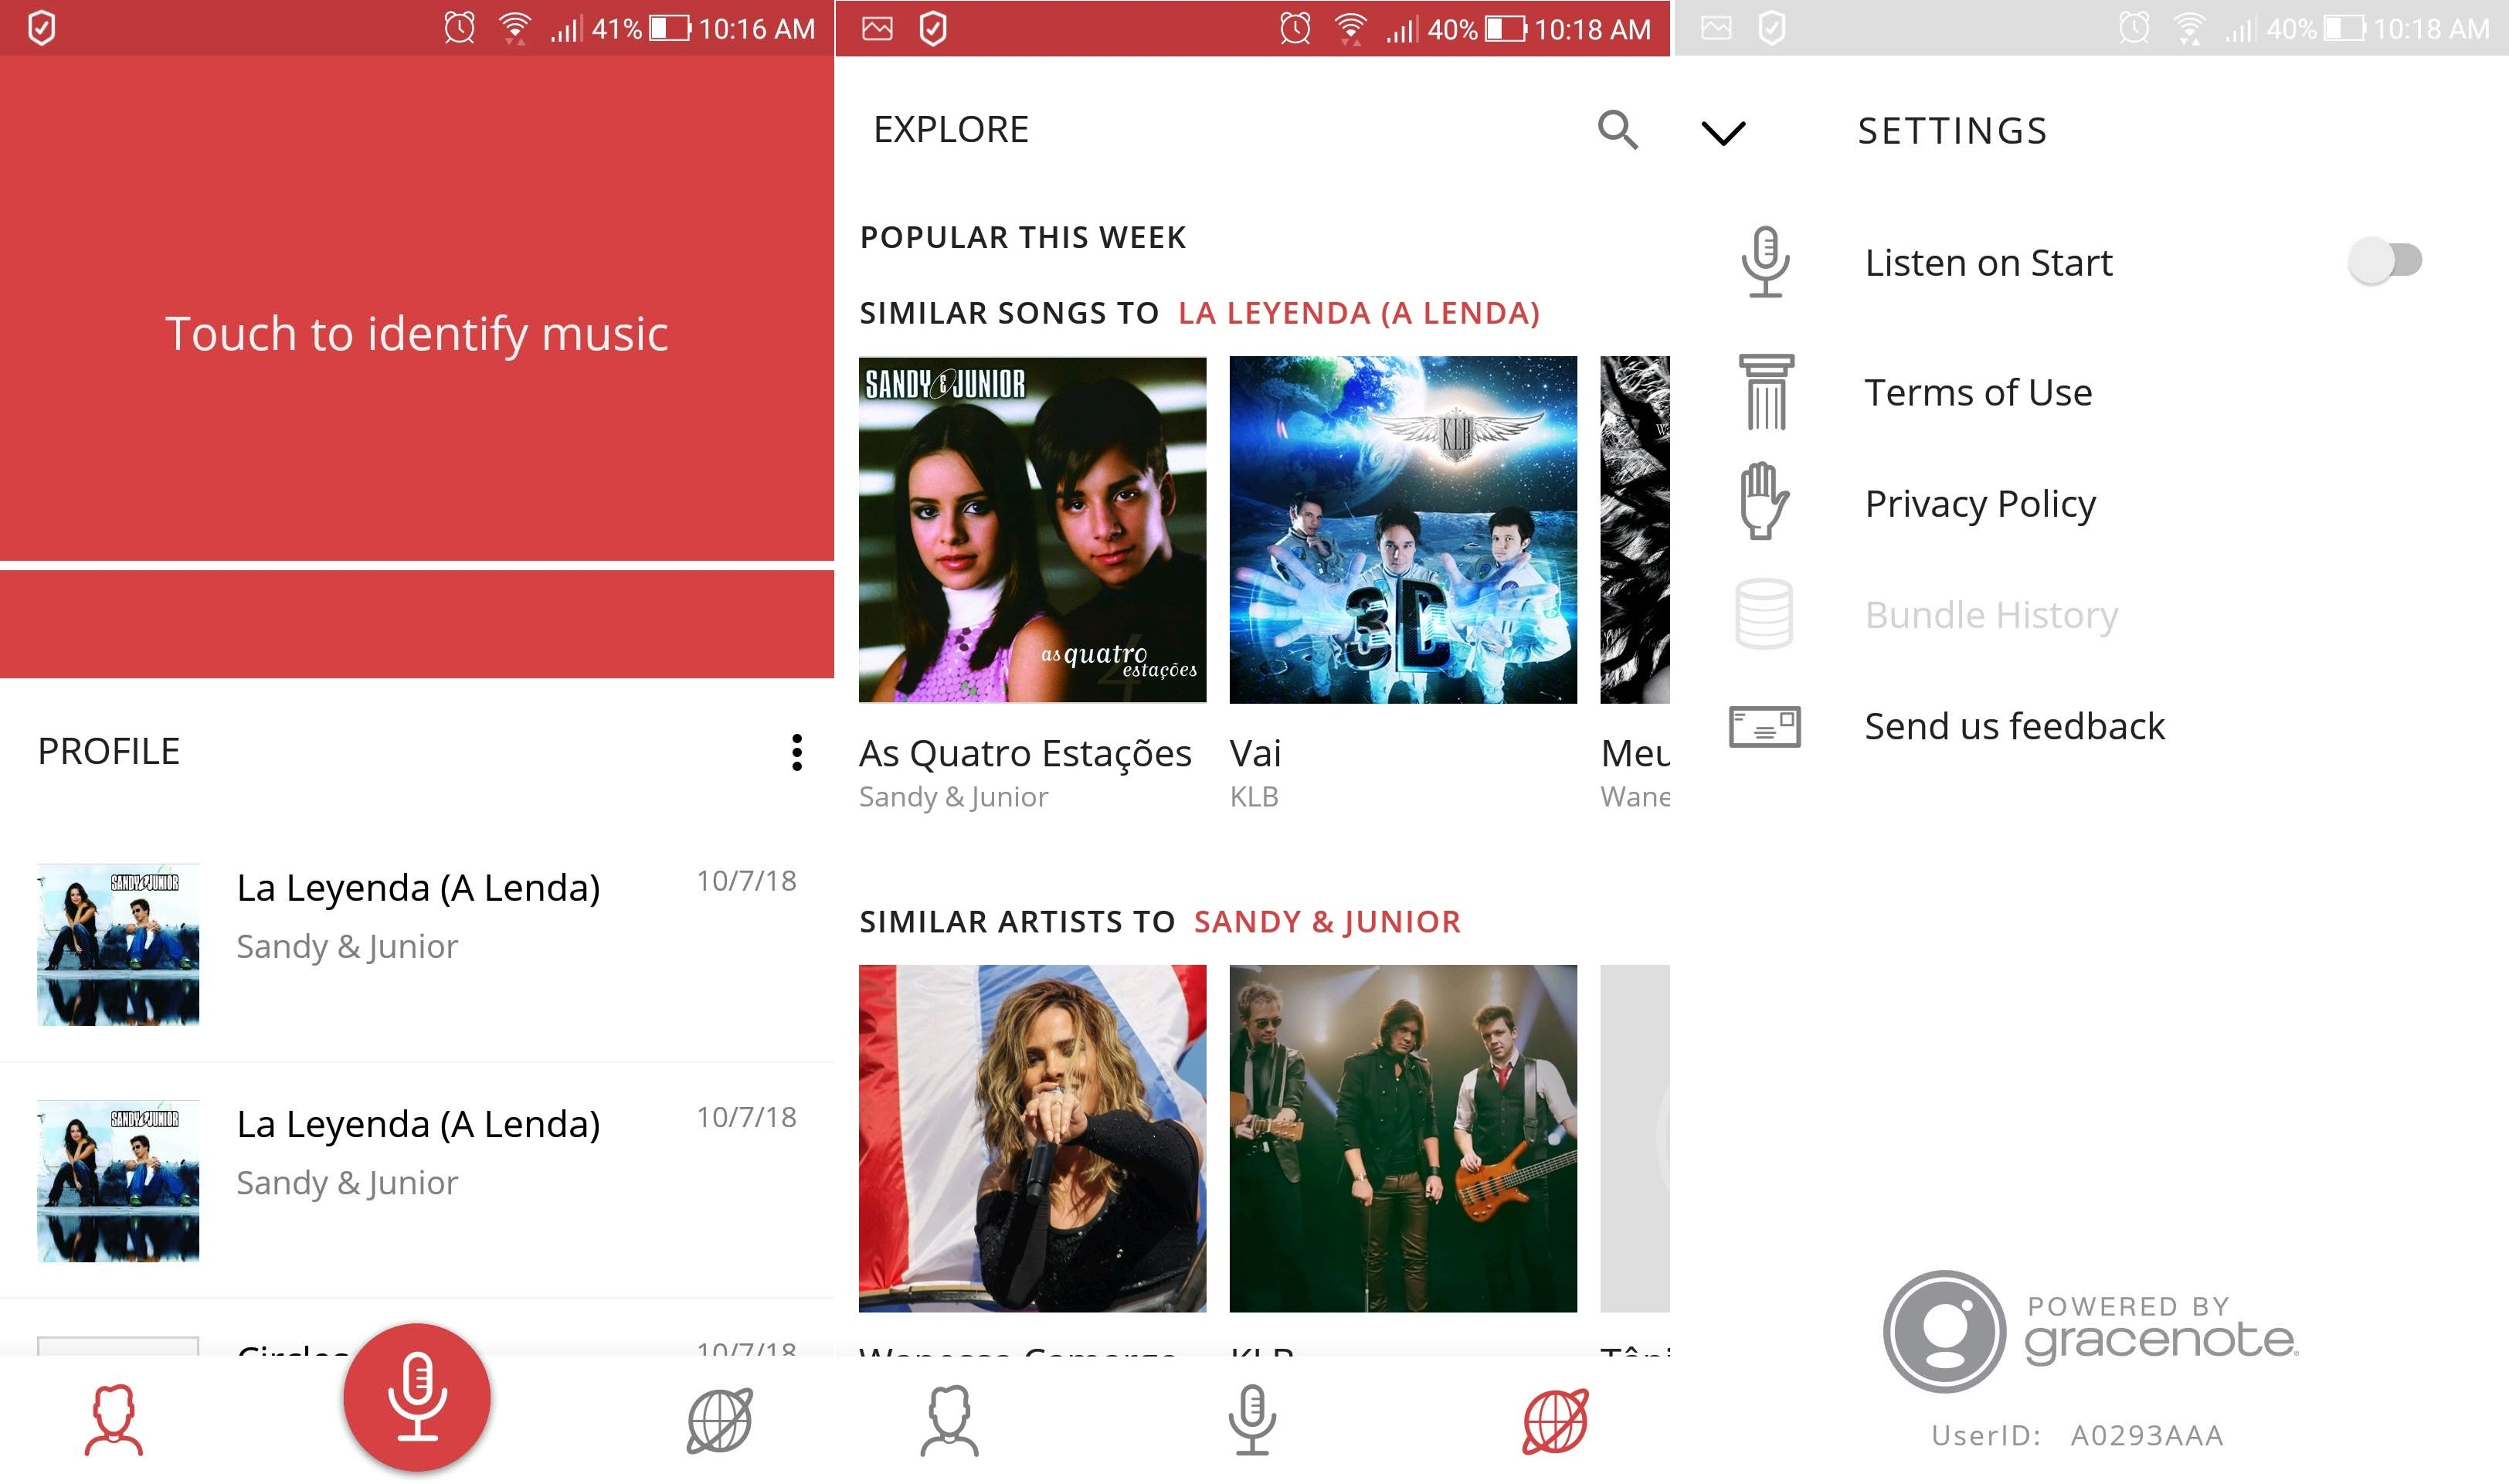
\includegraphics[scale=0.17]{figuras/MusicID.jpg}
   \\Fonte: Elaborado pela autora
\end{figure}

Segundo o site da companhia\footnote{http://www.gracenote.com/music/music-recognition/}, tradução nossa:

\begin{citacao}
O Gracenote MusicID\textregistered é o padrão para reconhecimento de música. Ele ajuda os fãs a desbloquear seus álbuns e faixas favoritos na nuvem e a descobrir novas músicas com seus celulares, além de permitir o monitoramento de músicas para detentores de direitos e profissionais do setor \cite{musicid1998}.
\end{citacao}

O Gracenote MusicID\textregistered, faz o reconhecimento de músicas que são tocadas ao seu redor, combinado ao uso de \textit{fingerprints} (ver subseção \ref{subsubsec:audioFingerprint}) e correspondência de texto para identificar arquivos de música digital em um banco de dados mundial de informações musicais. Uma vez reconhecidos, os arquivos são organizados por nome de faixa, nome do álbum e caminhos de pastas e, então, apresentados ao usuário. Ele é um aplicativo para \textit{smartphones} que identifica músicas ouvindo você cantar, cantarolar ou de músicas que são tocadas ao seu redor.

%SHAZAM%
\subsection{Shazam} \label{subsec:shazam}
\textit{Shazam Entertainment Ltd.} foi fundada em 2000 com a idéia de prover um serviço que pudesse conectar as pessoas à musica, permitindo a identificação da música através de \textit{smartphones}. A aplicação (ver Figura \ref{fig:shazam}) usa o microfone do \textit{smartphone} ou do computador para capturar uma pequena amostra de música e, então, realiza a identificação da música em um grande banco de dados com mais de 12 bilhões de músicas, com uma alta taxa de acertos.

\begin{figure}[!htb]
   \centering
   \caption{Shazam}\label{fig:shazam} 
   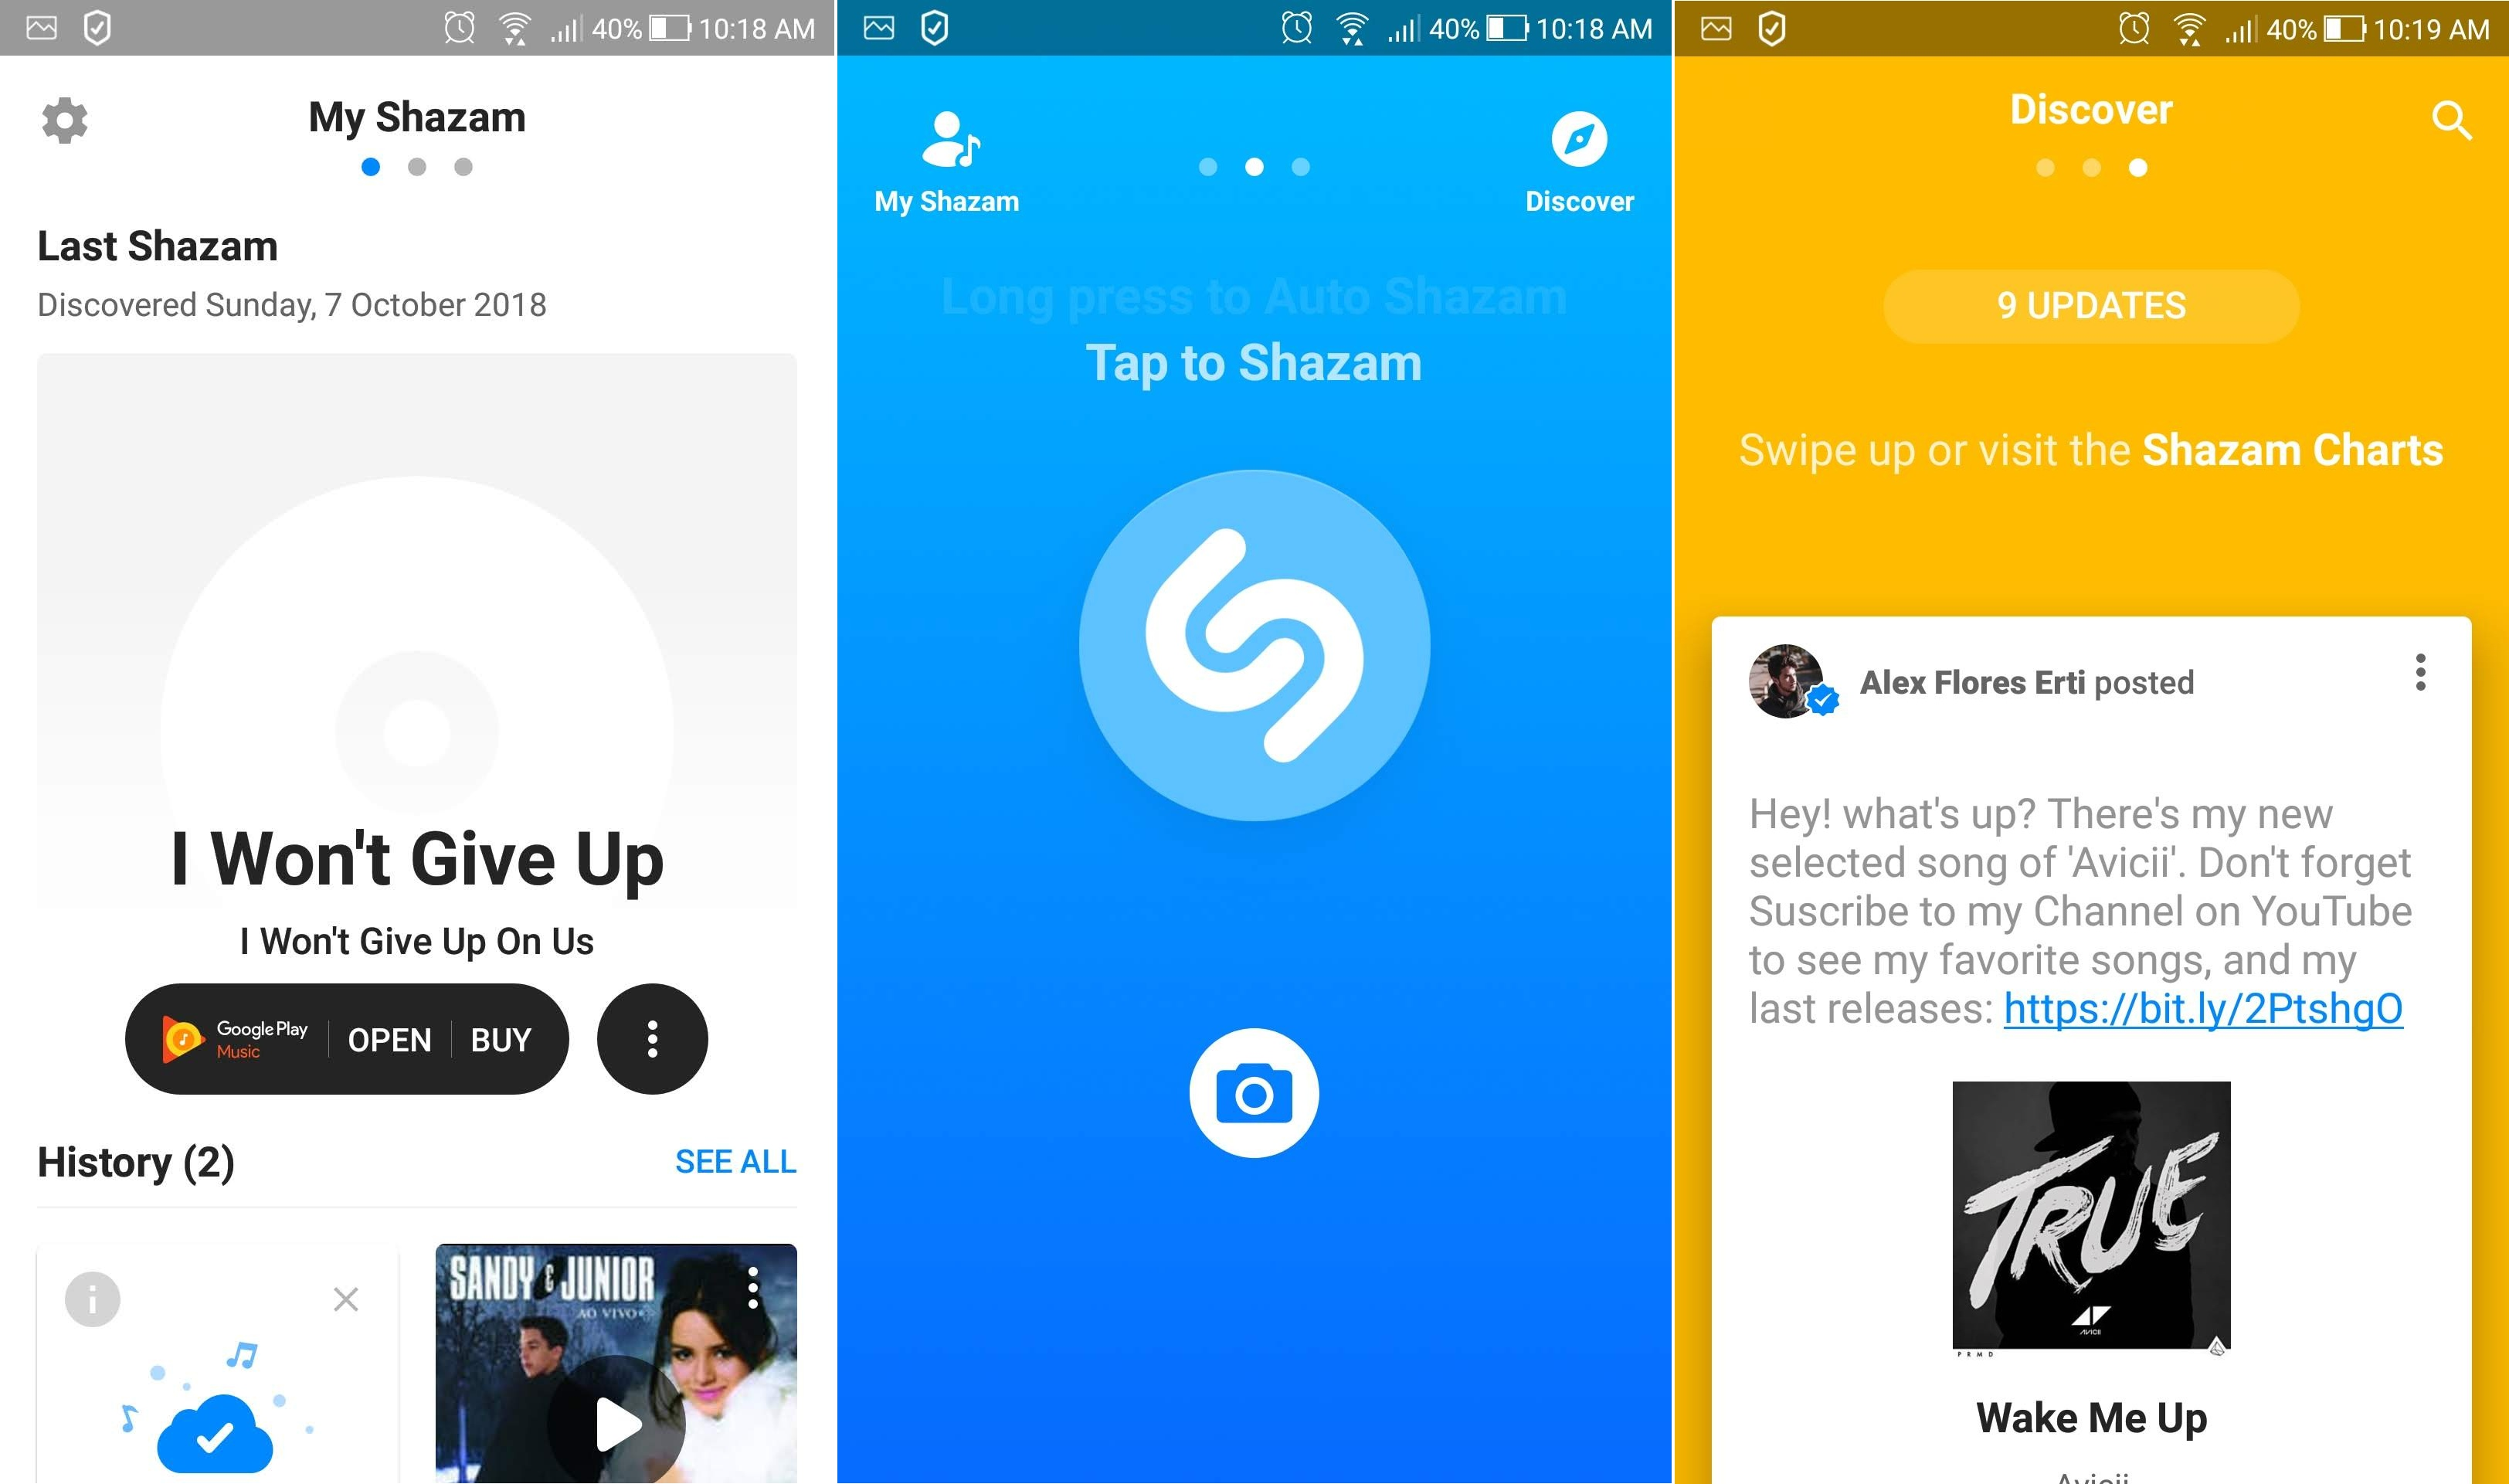
\includegraphics[scale=0.17]{figuras/shazam.jpg}
   \\Fonte: Elaborado pela autora
\end{figure}

Segundo o site da companhia\footnote{https://www.shazam.com/pt/company}:

\begin{citacao}
Shazam é uma aplicação móvel que reconhece música e conteúdos de TV à sua volta. É a melhor maneira de descobrir, explorar e compartilhar a música e os conteúdos de TV que você mais gosta. Levamos 10 anos para alcançar 1 bilhão de tags, 10 meses para chegar a 2 bilhões, 3 meses para ir de 10 a 12 bilhões... É uma aplicação fantástica, agora disponível nas lojas da Apple e Android. E estamos sempre à procura de novas maneiras de encantar os nossos usuários \cite{shazam2000}.
\end{citacao}

Para o trecho de música capturado pela aplicação é criado uma \textit{fingerprint} (ver subseção \ref{subsubsec:audioFingerprint}), que é comparada com todas as outras \textit{fingerprints} derivadas das músicas no banco de dados. Se houver uma correspondência, são enviadas informações da música para o usuário, como artista, álbum e título da música.

%SOUNDHOUND%
\subsection{SoundHound} \label{subsec:soundhound}
\textit{SoundHound Inc.}, fundada em 2005, é uma empresa pioneira em desenvolvimento de aplicações para reconhecimento de voz, compreensão da linguagem natural, reconhecimento de som e tecnologias de busca.

Segundo o site da companhia\footnote{https://soundhound.com/about}, tradução nossa:

\begin{citacao}
Acreditamos em permitir que humanos interajam com as coisas ao seu redor da mesma forma como interagimos entre nós: falando naturalmente com telefones celulares, carros, TVs, caixas de música, máquinas de café, e todas as outras partes emergentes do mundo "conectado". Nosso produto mais recente, Hound, utiliza a nossa tecnologia \textit{Speech-to-Meaning}\texttrademark\ para mostrar uma experiência inovadora com os \textit{Smartphones}. Nosso produto \textit{SoundHound} aplica nossa tecnologia a música, permitindo as pessoas descobrir, explorar e compartilhar música ao seu redor, e até mesmo encontrar o nome daquela música presa em suas cabeças cantando ou cantarolando. E através da plataforma Houndify, capacitamos os desenvolvedores para fazerem parte dessa revolução \textit{speech-to-meaning} \cite{soundhound2005}.
\end{citacao}

A plataforma independente de Inteligência Artificial \textit{Houndify}, combinada ao \textit{Automatic Speech Recognition} (ASR) e o \textit{Natural Language Understanding} (NLU), permite ao \textit{SoundHound} a identificação de músicas de forma rápida e eficiente. Seus dois produtos conhecidos no meio musical são:

\begin{enumerate}
    \item \textit{SoundHound Music Search \& Play}\footnote{https://soundhound.com/soundhound}: aplicativo para \textit{smartphones} onde é possível descobrir, pesquisar e reproduzir qualquer música com controle de voz (ver Figura \ref{fig:soundHound}). Ele é um aplicativo para \textit{smartphones} que identifica músicas ouvindo você cantar, cantarolar ou de músicas que são tocadas ao seu redor.
    \item \textit{Midomi}\footnote{https://www.midomi.com/}: aplicação com as mesmas características do item anterior, porém possui versão para \textit{web}. Sua  versão \textit{mobile} é destinada a modelos mais antigos de \textit{smartphones}.
\end{enumerate}

\begin{figure}[!htb]
   \centering
   \caption{SoundHound}\label{fig:soundHound} 
   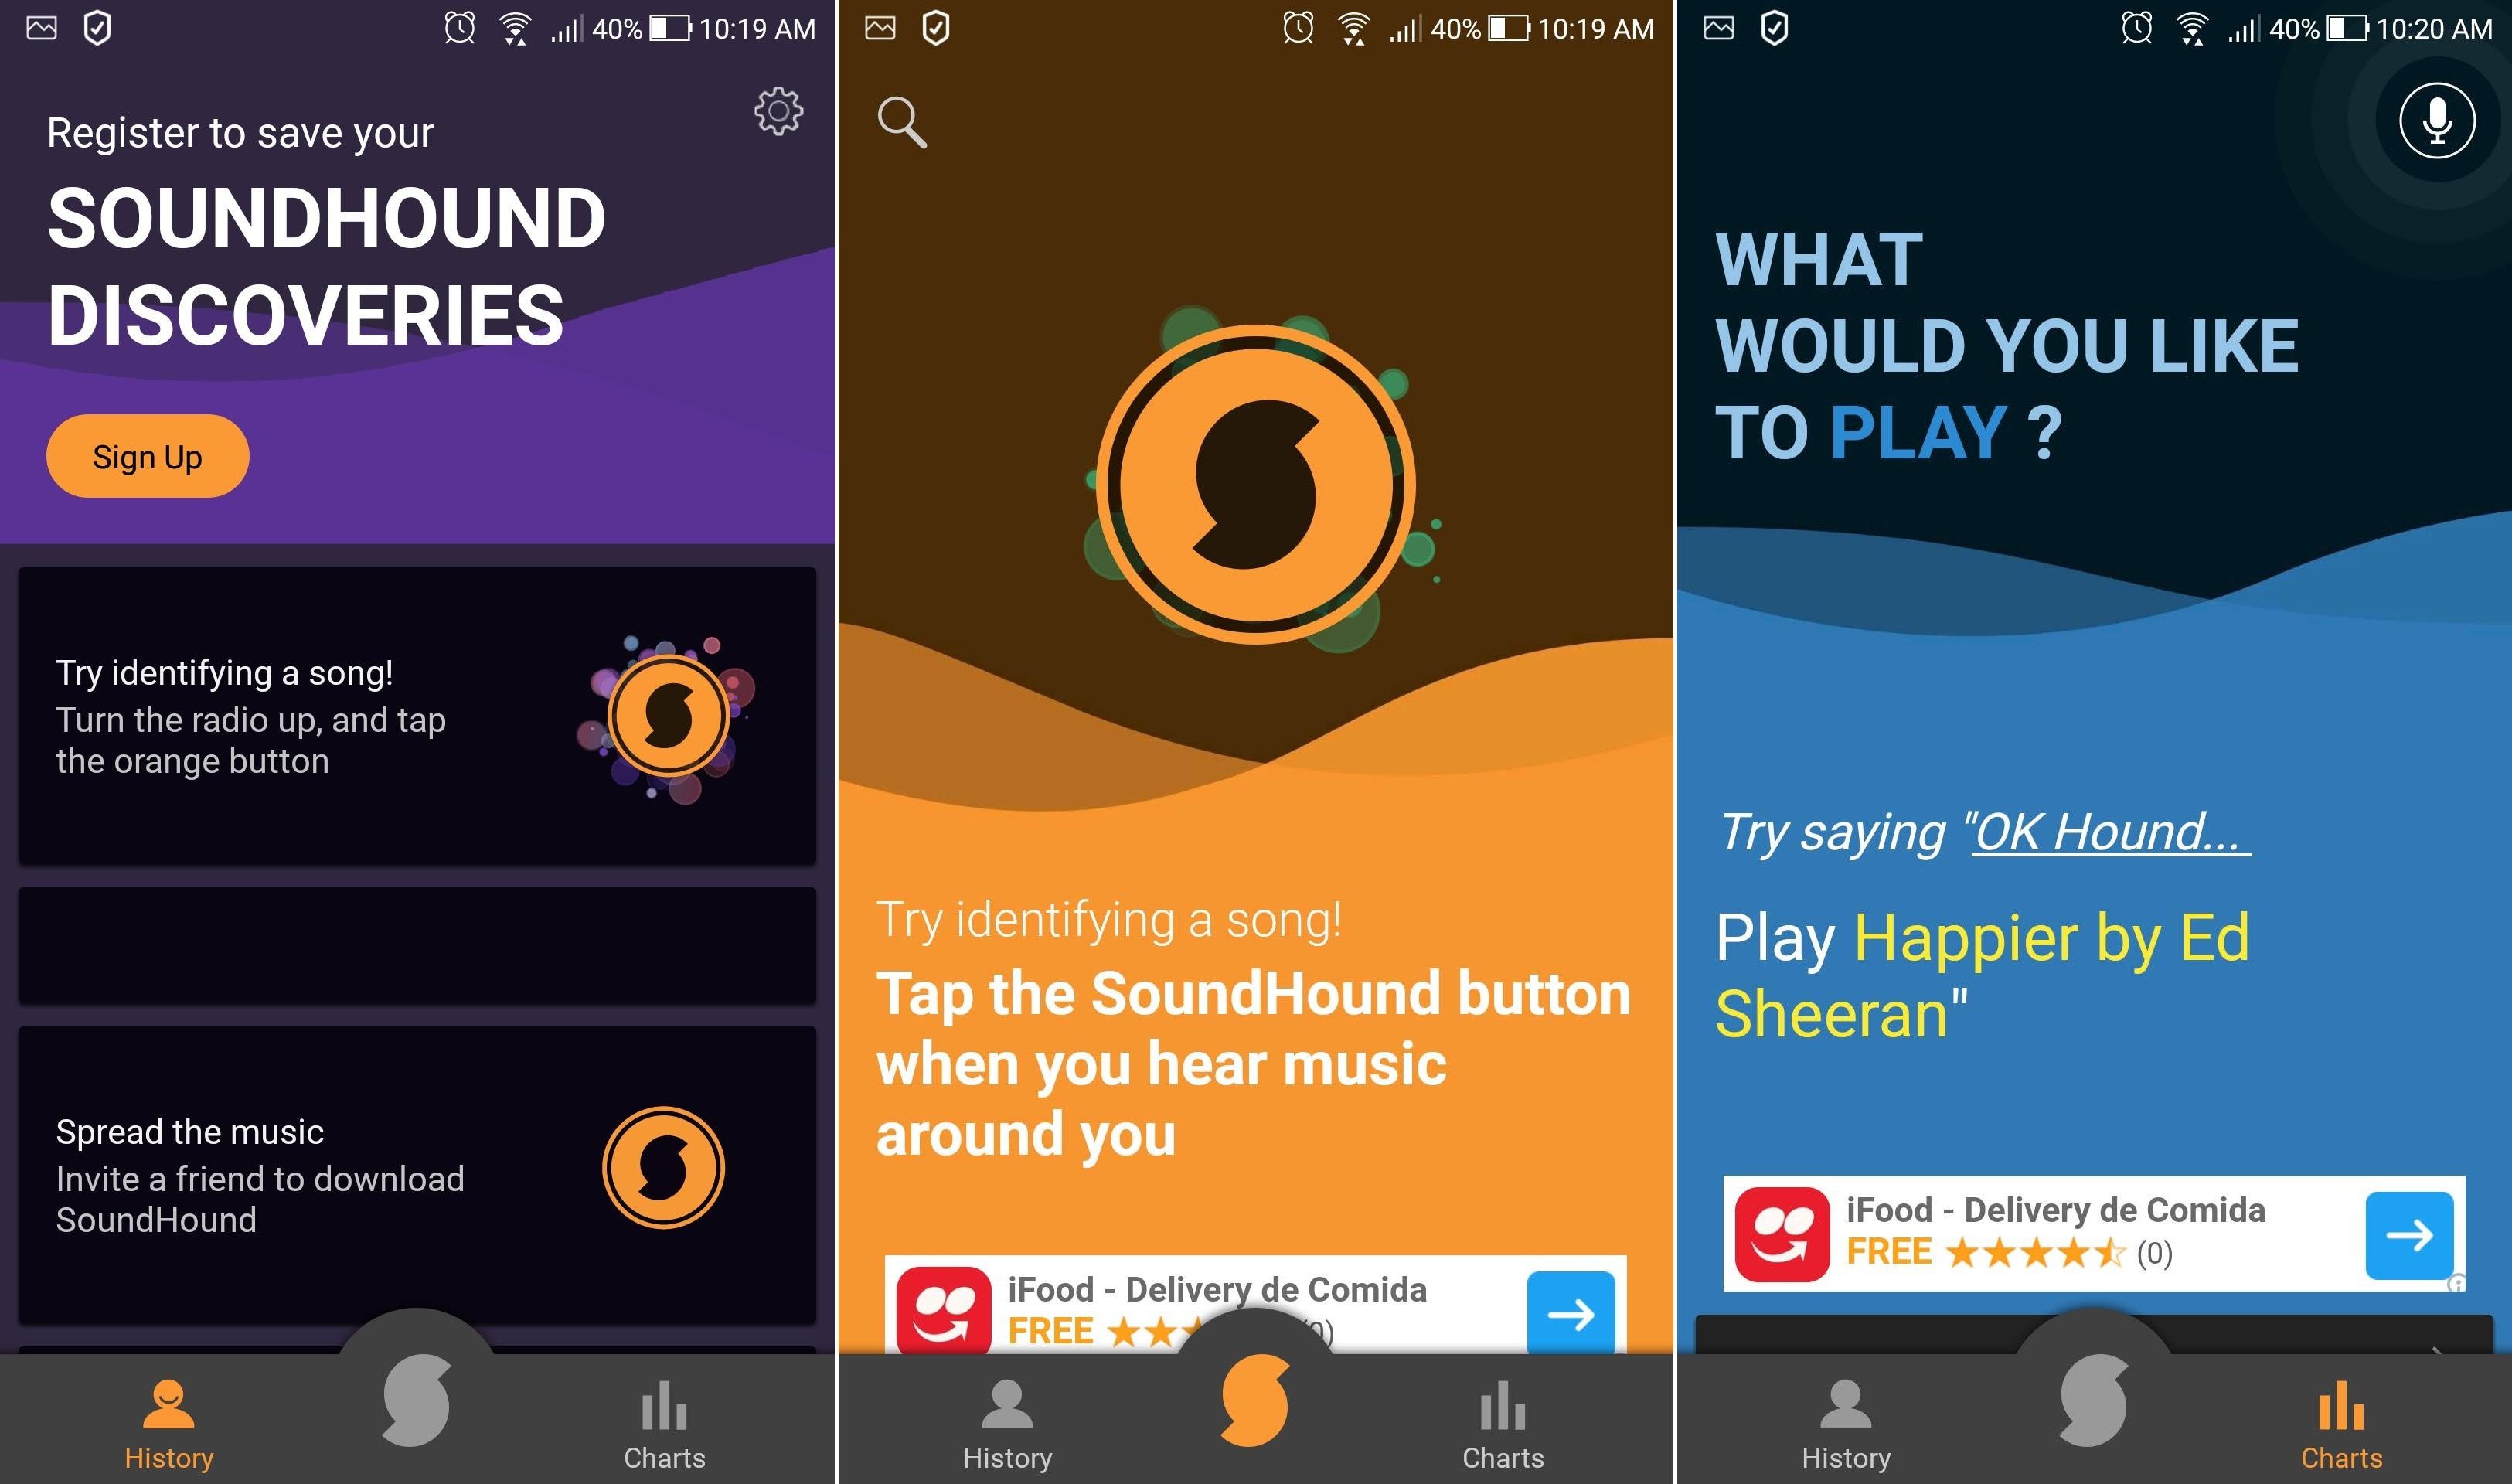
\includegraphics[scale=0.17]{figuras/soundhound.jpg}
   \\Fonte: Elaborado pela autora
\end{figure}

%DEEZER%
\subsection{Deezer} \label{subsec:deezer}
Esta solução nasceu da necessidade de facilitar a vida de seu fundador para ouvir e realizar o \textit{download} de músicas. Com isso, o idealizador da plataforma desenvolveu o \textit{Blogmusik.net} em 2006. Devido a sua popularidade, houve objeção de detentores de direitos autores, o que gerou o fechamento do site. Pouco tempo depois, um acordo foi assinado e o antigo site voltou ao ar com o nome de \textit{Deezer} (ver Figura \ref{fig:deezer}).

\begin{figure}[!htb]
   \centering
   \caption{Deezer}\label{fig:deezer} 
   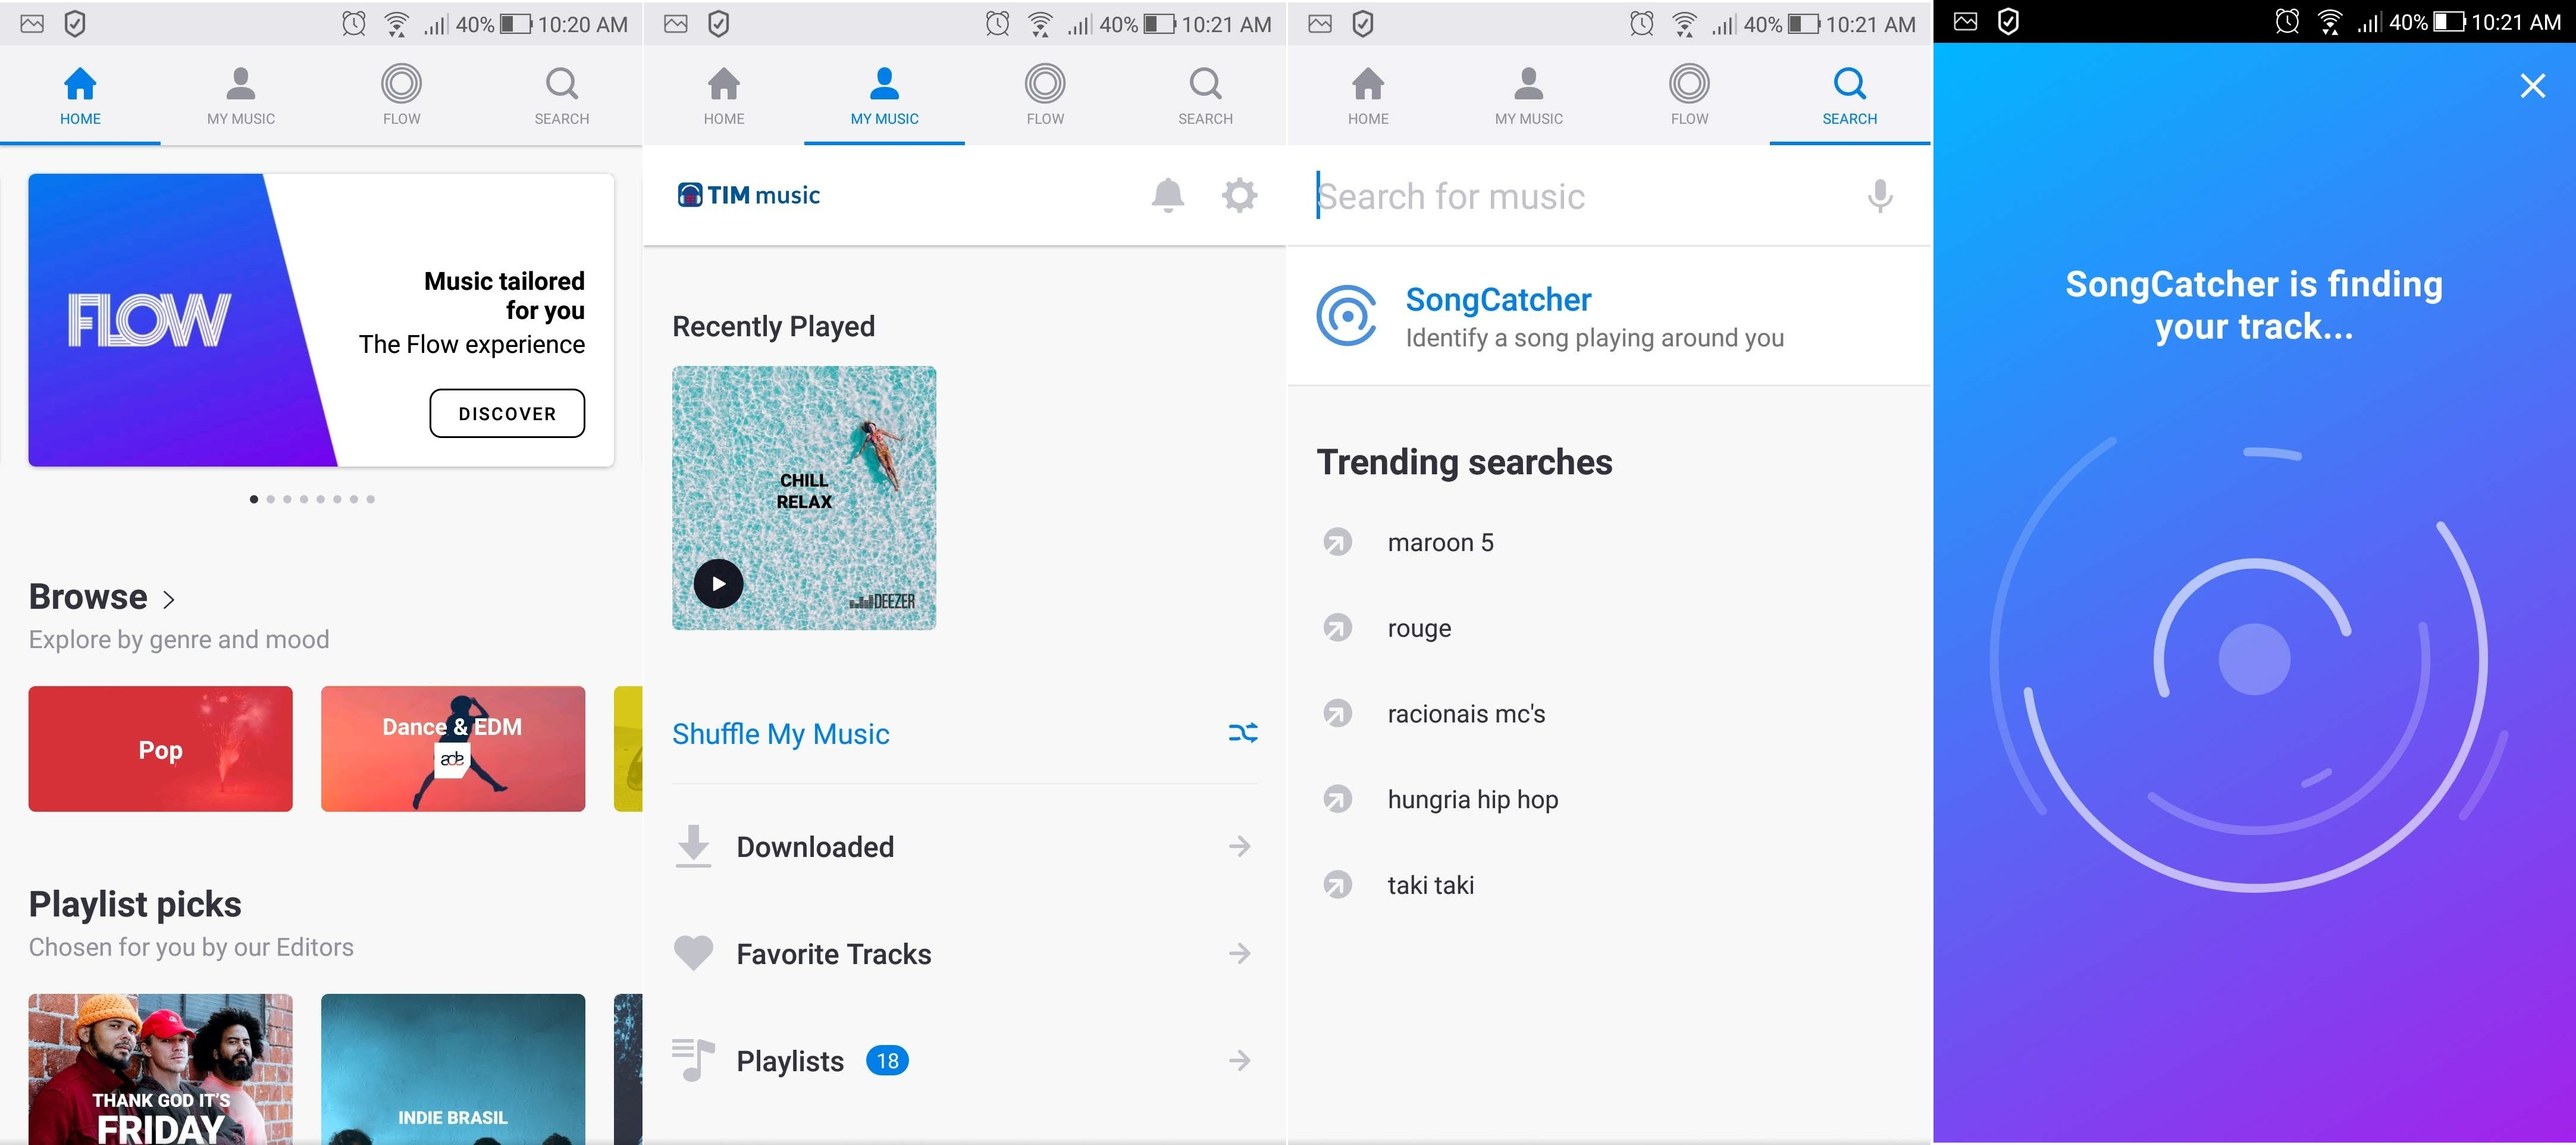
\includegraphics[scale=0.13]{figuras/deezer.jpg}
   \\Fonte: Elaborado pela autora
\end{figure}

Segundo o site da companhia\footnote{https://www.deezer.com/br/company}:

\begin{citacao}
Na Deezer você ouve toda e qualquer música, na hora que quiser. Explore mais de 53 milhões de faixas (e a contagem continua) e descubra artistas e músicas que você vai amar com a recomendação personalizada dos Editores Deezer. A Deezer está em todos os seus dispositivos, tanto on-line como off-line, sem limites de escuta. Música na ponta de seus dedos para todos os momentos do seu dia: amanhecer, ir ao trabalho, relaxar, viver a vida...é só dar play! \cite{deezer2006}
\end{citacao}

A Deezer (ver Figura \ref{fig:deezer}), também conta com uma série de aplicativos que complementam a experiência musical do usuário. O \textit{Stateeztics}, por exemplo, é um \textit{in-app} exclusivo que traça o perfil musical do usuário e mostra suas estatísticas de consumo a partir do seu histórico sonoro. Outra aplicação disponível é o \textit{Edjing}, que oferece mixagem de músicas com diversas ferramentas de efeitos digitais, além de contar com uma interface bastante intuitiva. Já o usuário que está aprendendo a tocar instrumentos musicais pode contar com o \textit{Chordify}, que reconhece o som que está tocando na Deezer e faz a transcrição automática da harmonia em cifras.

Recentemente, no final do ano de 2017, além da correspondência de texto para identificar arquivos de música digital, a Deezer lançou o seu próprio recurso de identificação de músicas que são tocadas ao seu redor combinado ao uso de \textit{fingerprints}, o \textit{SongCatcher}, desenvolvido pela \textit{ACRCloud} (ver subseção \ref{subsec:acrcloud}).

%SPOTIFY%
\subsection{Spotify} \label{subsec:spotify}
\textit{Spotify Ltd.}, fundada em 2006, é um serviço de \textit{streaming} de música, \textit{podcast} e vídeo, além de ser o mais usado no mundo. A plataforma fornece conteúdo protegido provido de restrição pela gestão de direitos digitais de gravadoras e empresas de mídia (ver Figura \ref{fig:spotify}). O Spotify é um serviço \textit{freemium}: ele possui recursos gratuitos com propagandas ou limitações, e recursos adicionais, como qualidade de transmissão aprimorada e \textit{downloads} de música, que são oferecidos para assinaturas pagas.

\begin{figure}[!htb]
   \centering
   \caption{Spotify}\label{fig:spotify} 
   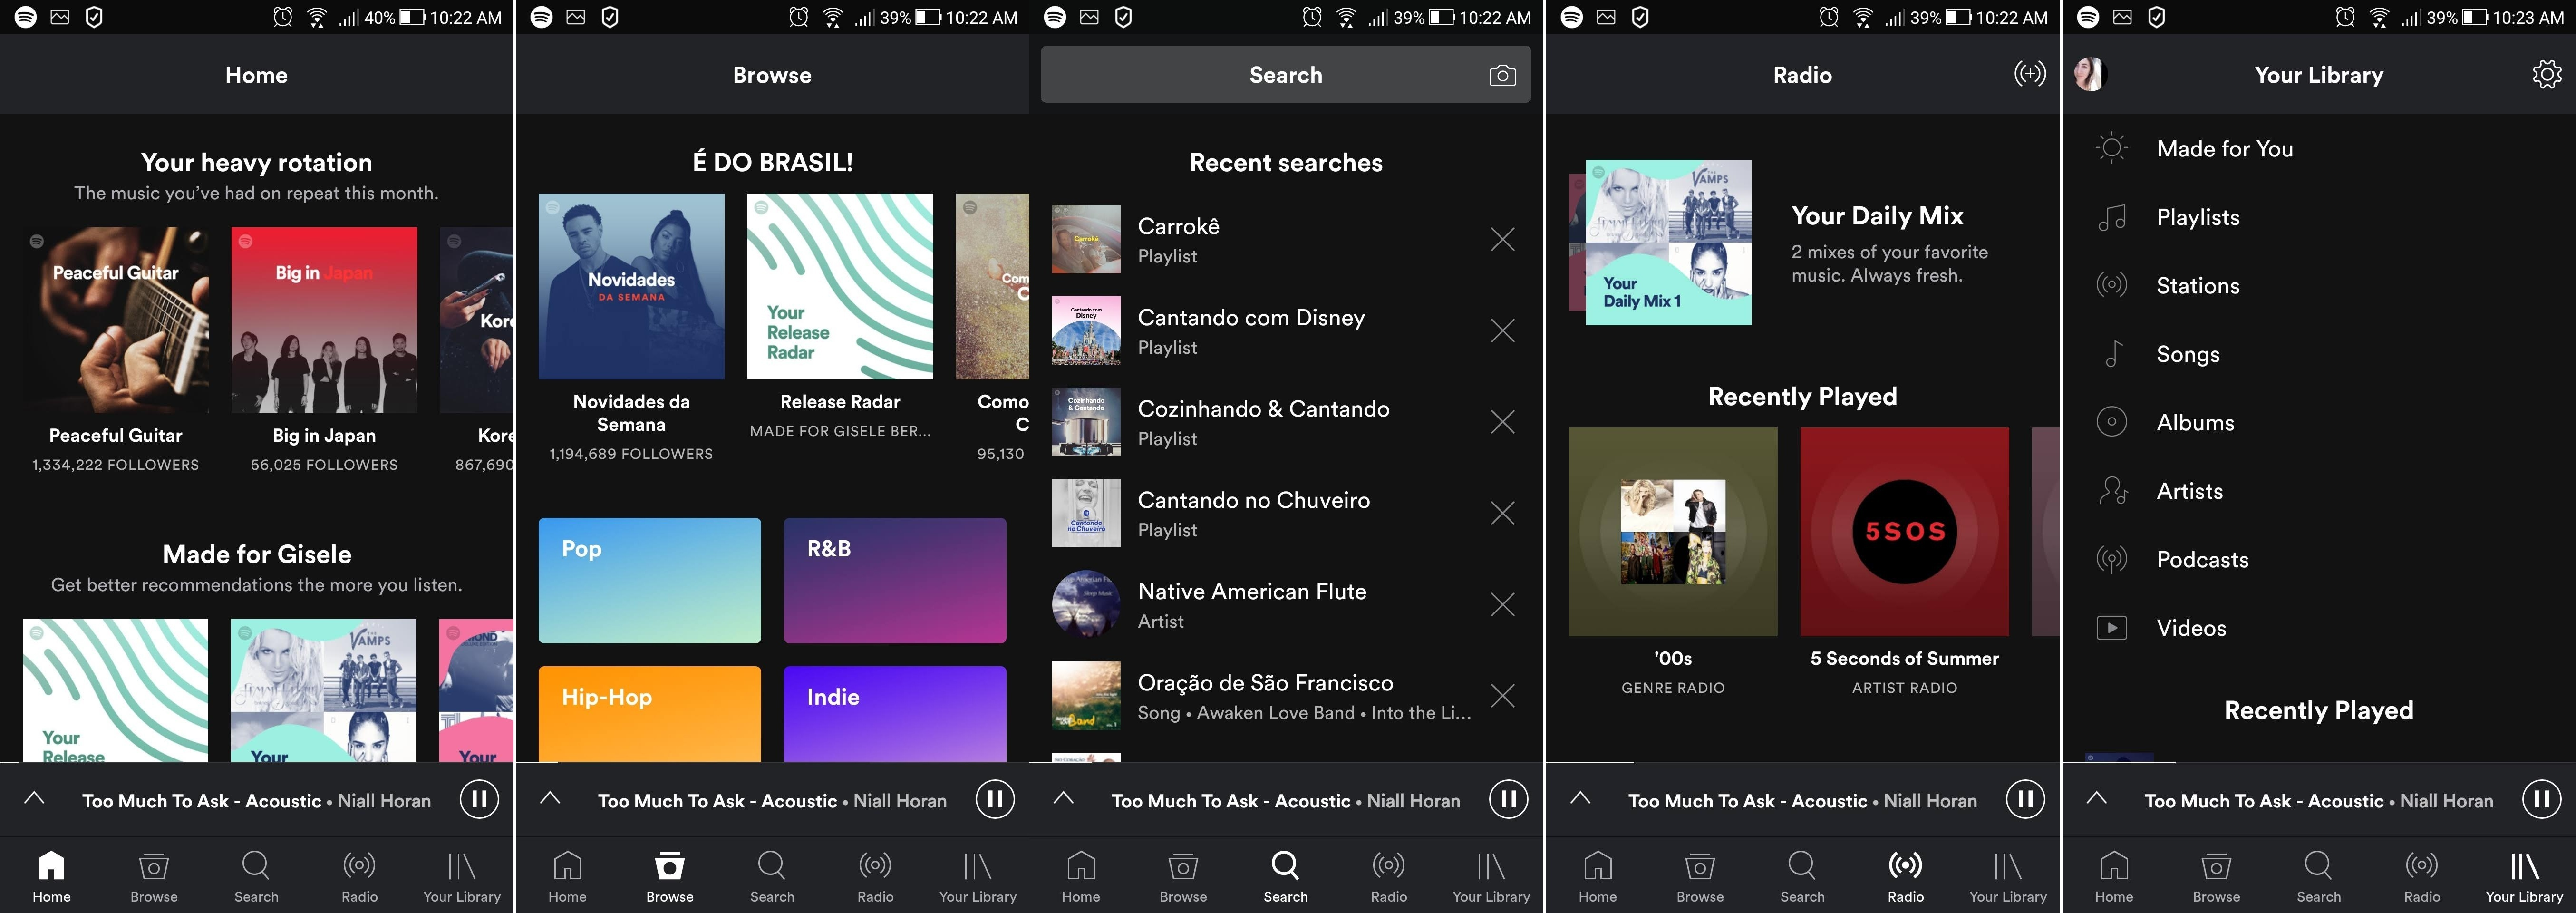
\includegraphics[scale=0.10]{figuras/spotify.jpg}
   \\Fonte: Elaborado pela autora
\end{figure}

Segundo o site da companhia\footnote{https://www.spotify.com/br/about-us/contact/}:

\begin{citacao}
Com o Spotify, é fácil encontrar a música certa para cada momento – no seu telefone, computador, tablet e outros. Existem milhões de faixas no Spotify. Não importa se você está malhando, em uma festa ou relaxando, a música certa está sempre em suas mãos. Escolha o que quer ouvir ou deixe o Spotify surpreendê-lo. Você também pode navegar pelas coleções de músicas de amigos, artistas e celebridades, ou criar uma estação de rádio e simplesmente aproveitar. Produza a trilha sonora de sua vida com o Spotify. Assine ou ouça de graça \cite{spotify2006}.
\end{citacao}

A plataforma emprega um modelo de distribuição de dados híbrido com uma combinação de compartilhamento de dados peer-to-peer\footnote{Do inglês par-a-par ou simplesmente ponto-a-ponto, é uma arquitetura de redes de computadores onde cada um dos pontos ou nós da rede funciona tanto como cliente quanto como servidor, permitindo compartilhamentos de serviços e dados sem a necessidade de um servidor central.} (P2P) e uma infraestrutura de servidor. Ao pesquisar uma música através do smartphone e querer ouvi-lá, o sistema irá primeiro verificar se a música já se encontra baixada na memória cache do \textit{smartphone} para agilizar o processo, em caso negativo é feita a conexão diretamente com o servidor do Spotify, ao mesmo tempo que o método busca "peers"\ entre milhões de usuários para que a música que se queira ouvir, seja baixada o mais rápido possível. A busca da música é feita pela correspondência de texto para identificar arquivos de música digital através da técnica de recuperação por conteúdo (ver subseção \ref{subsubsec:rpc}).

O Spotify disponibiliza uma \textit{Web API}\footnote{Do termo em inglês "Application Programming Interface"\ que significa em tradução para o português "Interface de Programação de Aplicativos". É uma forma de integrar sistemas, possibilitando benefícios como a facilidade no intercâmbio entre informações com diferentes linguagens de programação.} que permite que desenvolvedores integrem o conteúdo do Spotify em seus próprios aplicativos. O Spotify \textit{Web API} é um serviço com base na arquitetura REST, que retorna em formato JSON dados sobre álbuns, artistas, faixas, playlists, entre outros. Para acessar outras informações é necessária uma autenticação \textit{OAuth}.

%===>>> RONALDO - 23/10/2018: AQUI NO SPOTIFY TAMBEM SENTI FALTA DA EXPLICACAO DA TECNICA USADA PARA BUSCA POR SIMILARIDADE
%===>>> GISELE - 24/10/2018: O SPOTIFY USA PEER-TO-PEER PARA BUSCA DA MÚSICA, E É PELA RECUPERAÇÃO DE CONTEÚDO, USANDO APENAS METADADOS.
%===>>> RONALDO - 29/10/2018: SUGIRO COLOCAR ESSA EXPLICACAO TUA ACIMA NO FINAL DO PARÁGRAFO QUE FALA SOBRE P2P. ELE FAZ ENTAO SOMENTE BUSCA EXATA USANDO OS METADADOS? DEIXAR ISSO CLARO NESTA EXPLICACAO...
%===>>> GISELE - 29/10/2018: AJUSTADO EXPLICAÇÃO. VÊ SE FICOU MELHOR.

%SOUNDCLOUD%
\subsection{SoundCloud} \label{subsec:soundcloud}
\textit{SoundCloud}, criada em 2007, é uma plataforma on-line de publicação de áudio utilizada por profissionais de música (ver Figura \ref{fig:soundcloud}). Nela os músicos podem colaborar, compartilhar, promover e distribuir suas composições.
Originalmente, seu objetivo era permitir que profissionais da música trocassem ideias sobre as composições nas quais estão trabalhando, permitindo uma fácil colaboração e comunicação antes de um lançamento público. Hoje, o site também é utilizado por ouvintes e usuários da \textit{web} em geral.

\begin{figure}[!htb]
   \centering
   \caption{SoundCloud}\label{fig:soundcloud} 
   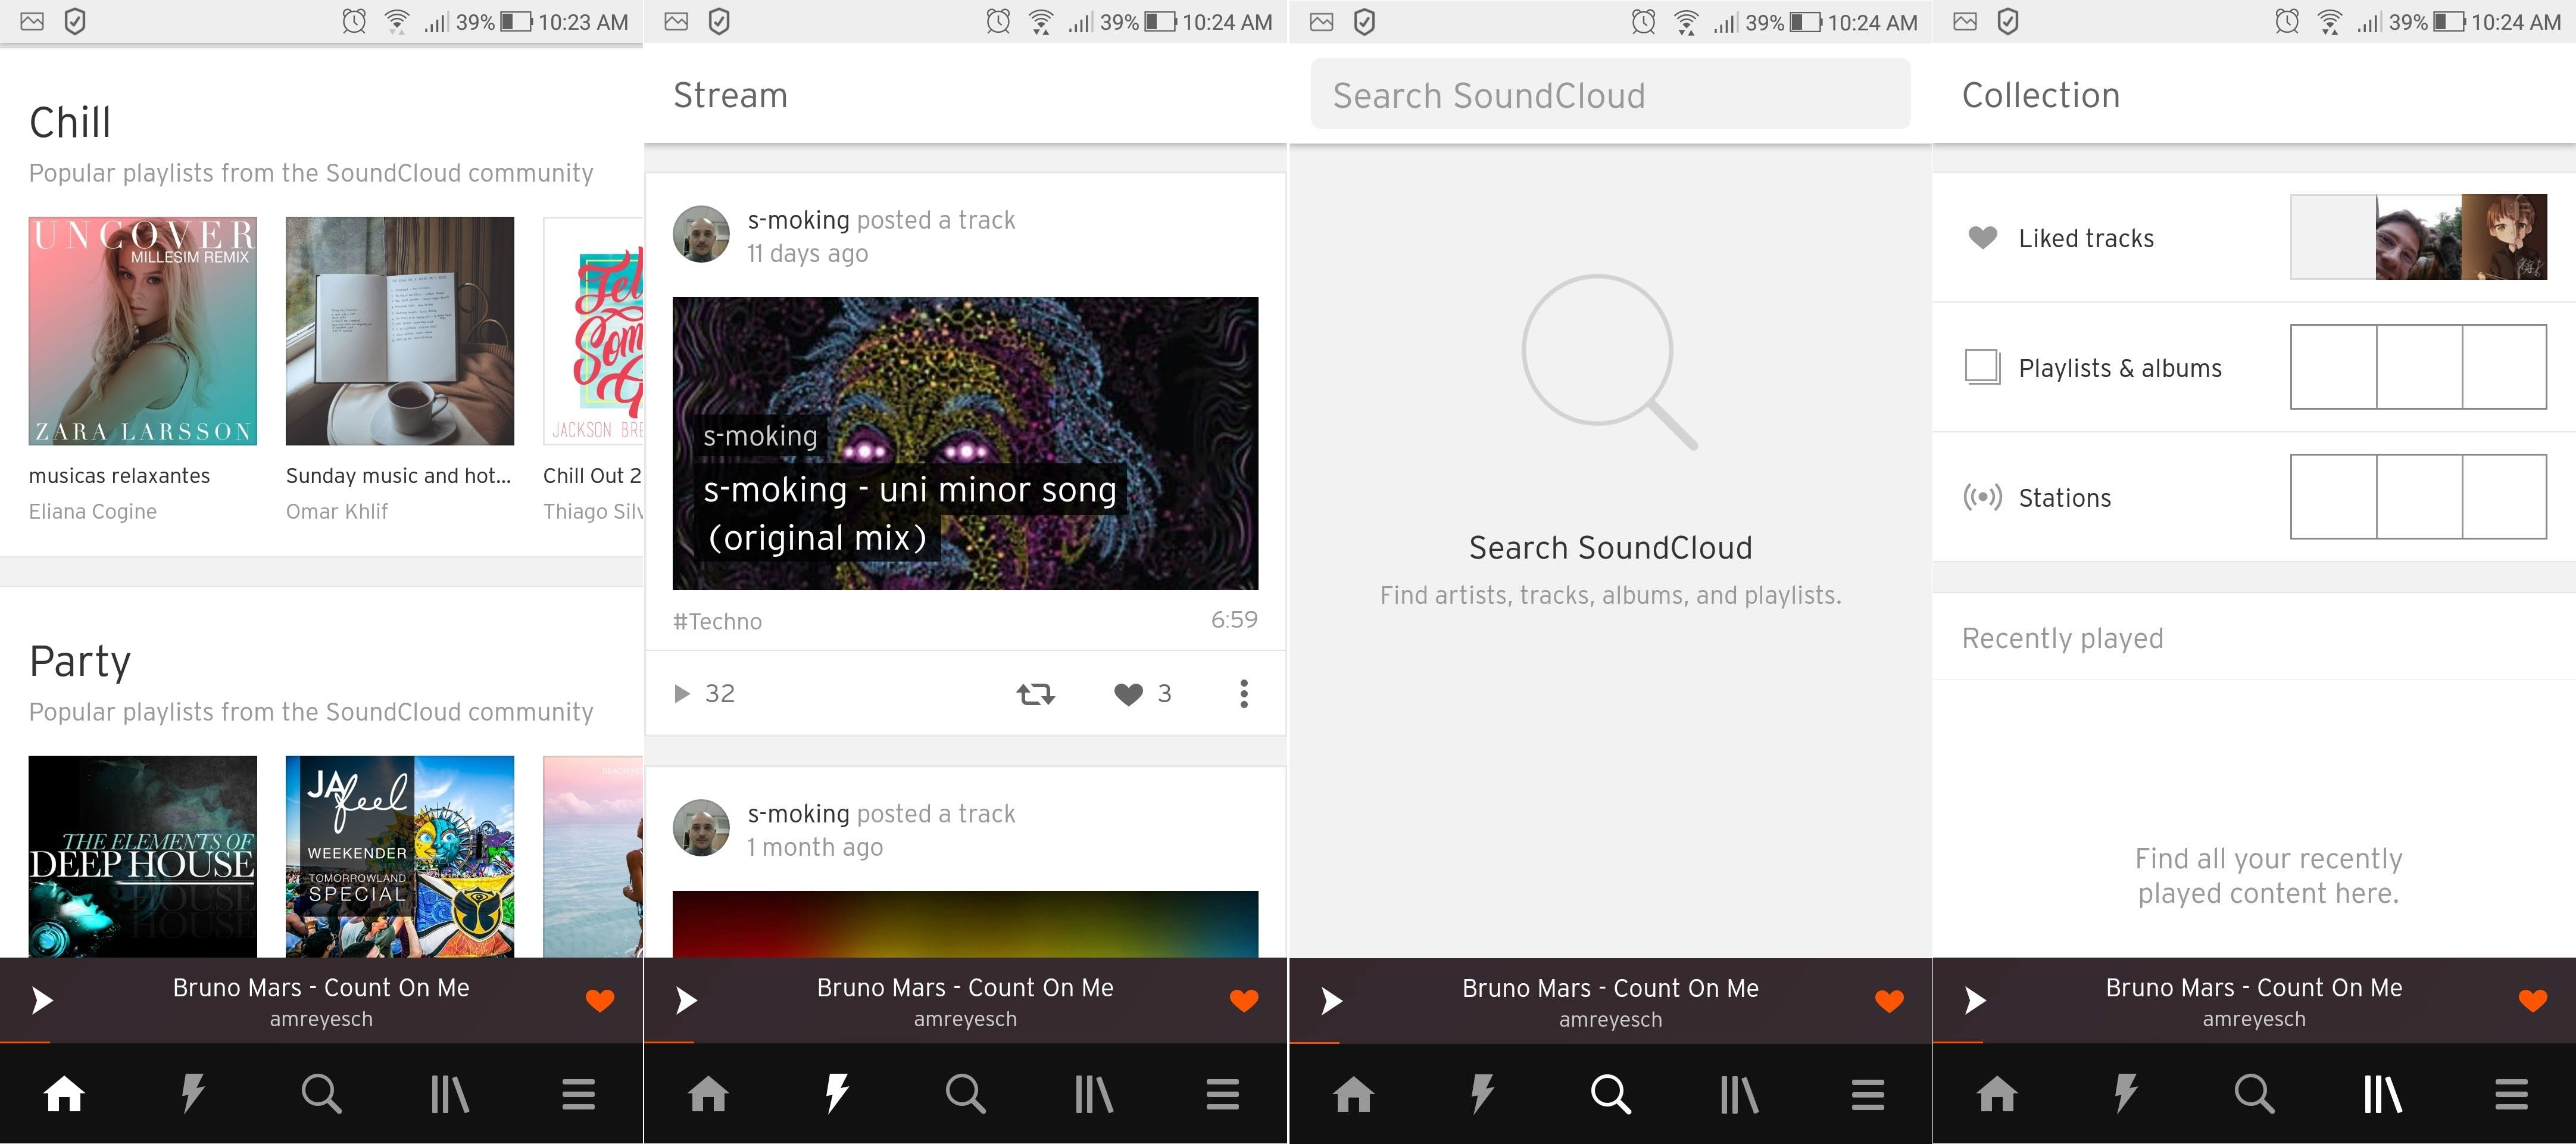
\includegraphics[scale=0.12]{figuras/soundcloud.jpg}
   \\Fonte: Elaborado pela autora
\end{figure}

Segundo o site da companhia\footnote{https://soundcloud.com/pages/contact}, tradução nossa:

\begin{citacao}
Como a maior plataforma de música e áudio do mundo, o SoundCloud permite que as pessoas descubram e desfrutem da maior seleção de músicas da mais diversificada comunidade de criadores do mundo. Desde o seu lançamento em 2008, a plataforma tornou-se famosa por seu conteúdo e recursos exclusivos, incluindo a capacidade de compartilhar músicas e se conectar diretamente com artistas, bem como descobrir trilhas inovadoras, demonstrações brutas, \textit{podcasts} e muito mais. Isso é possível graças a uma plataforma aberta que conecta diretamente os criadores e seus fãs em todo o mundo. Os criadores de música e áudio usam o SoundCloud para compartilhar e gerar receita com seu conteúdo com um público global, além de receber estatísticas detalhadas e \textit{feedback} da comunidade do SoundCloud. Ainda não tem uma conta gratuita? \cite{soundcloud2007}
\end{citacao}

Os usuários registrados podem ouvir o máximo de conteúdo como quiserem e podem fazer o \textit{upload} de até 180 minutos de áudio ao seu perfil. Todos esses recursos são gratuitos e estão disponíveis para todos os usuários registrados. A plataforma possui uma API integrada a várias aplicações, que permitem fazer o \textit{upload} ou \textit{download} de música e arquivos de música.

O SoundCloud descreve as faixas de música graficamente como formas de onda e permite aos usuários comentar partes específicas do áudio (conhecido como comentários cronometrados). Estes comentários são exibidos ao escutar a parte do áudio que estão se referindo. Outras características incluem respostas, listas de reprodução, seguidores e \textit{downloads} digitais de cortesia. A busca da música é feita pela correspondência de texto para identificar arquivos de música digital através da técnica de recuperação por conteúdo (ver subseção \ref{subsubsec:rpc}). Não foi encontrado documentação informando como funciona a recuperação da música.

O SoundCloud também disponibiliza uma \textit{Web API} que permite que desenvolvedores integrem o conteúdo do SoundCloud em seus próprios aplicativos. O SoundCloud \textit{Web API} é um serviço com base na arquitetura HTTP, que retorna em formato JSON dados sobre álbuns, artistas, faixas, playlists, entre outros. Para acessar outras informações é necessária uma autenticação \textit{OAuth}.

%===>>> RONALDO - 23/10/2018: AQUI NO SOUNDCLOUD TAMBEM SENTI FALTA DA EXPLICACAO DA TECNICA USADA PARA BUSCA POR SIMILARIDADE
%===>>> GISELE - 24/10/2018: DA MESMA FORMA QUE O SPOTIFY, É POR RECUPERAÇÃO POR CONTEÚDO, ONDE VOCÊ BUSCA A MÚSICA POR METADADOS. NÃO ENCONTREI DOCUMENTAÇÃO INFORMANDO COMO FUNCIONA A RECUPERAÇÃO DA MÚSICA DO SOUNDCLOUD.
%===>>> RONALDO - 29/10/2018: COMENTAR ENTAO, AO FINAL DO PENULTIMO PARAGRAFO ACIMA, QUE A BUSCA EH FEITA PELOS METADADOS
%===>>> GISELE - 29/10/2018: AJUSTADO EXPLICAÇÃO. VÊ SE FICOU MELHOR.

%MUSIXMATCH%
\subsection{Musixmatch} \label{subsec:musixmatch}
A \textit{Musixmatch} foi criada em 2010 com o objetivo de mudar a forma como as pessoas experimentam música e letras. Segundo o site da companhia\footnote{http://about.musixmatch.com/}, tradução nossa:

\begin{citacao}
Musixmatch é a maior plataforma de letras do mundo - onde você pode pesquisar, curtir e compartilhar letras de qualquer música, em qualquer lugar do mundo \cite{musixmatch2010}.
\end{citacao}

A plataforma pode ser acessada através do site ou via aplicativo para \textit{smartphones} (ver Figura \ref{fig:musixmatch}). O Musixmatch digitaliza todas as músicas da biblioteca de música do usuário e encontra letras para todas elas, identificando a letra da música e mantendo sincronizada enquanto a música é tocada. Além da correspondência de texto para identificar arquivos de música digital através da técnica de recuperação por conteúdo (ver subseção \ref{subsubsec:rpc}), ela possui também a capacidade para capturar uma pequena amostra de música através de \textit{fingerprints} (mesma função encontrada em soluções como o \textit{Shazam}), desenvolvido pela ACRCloud (ver subseção \ref{subsec:acrcloud}).

\begin{figure}[!htb]
   \centering
   \caption{Musixmatch}\label{fig:musixmatch} 
   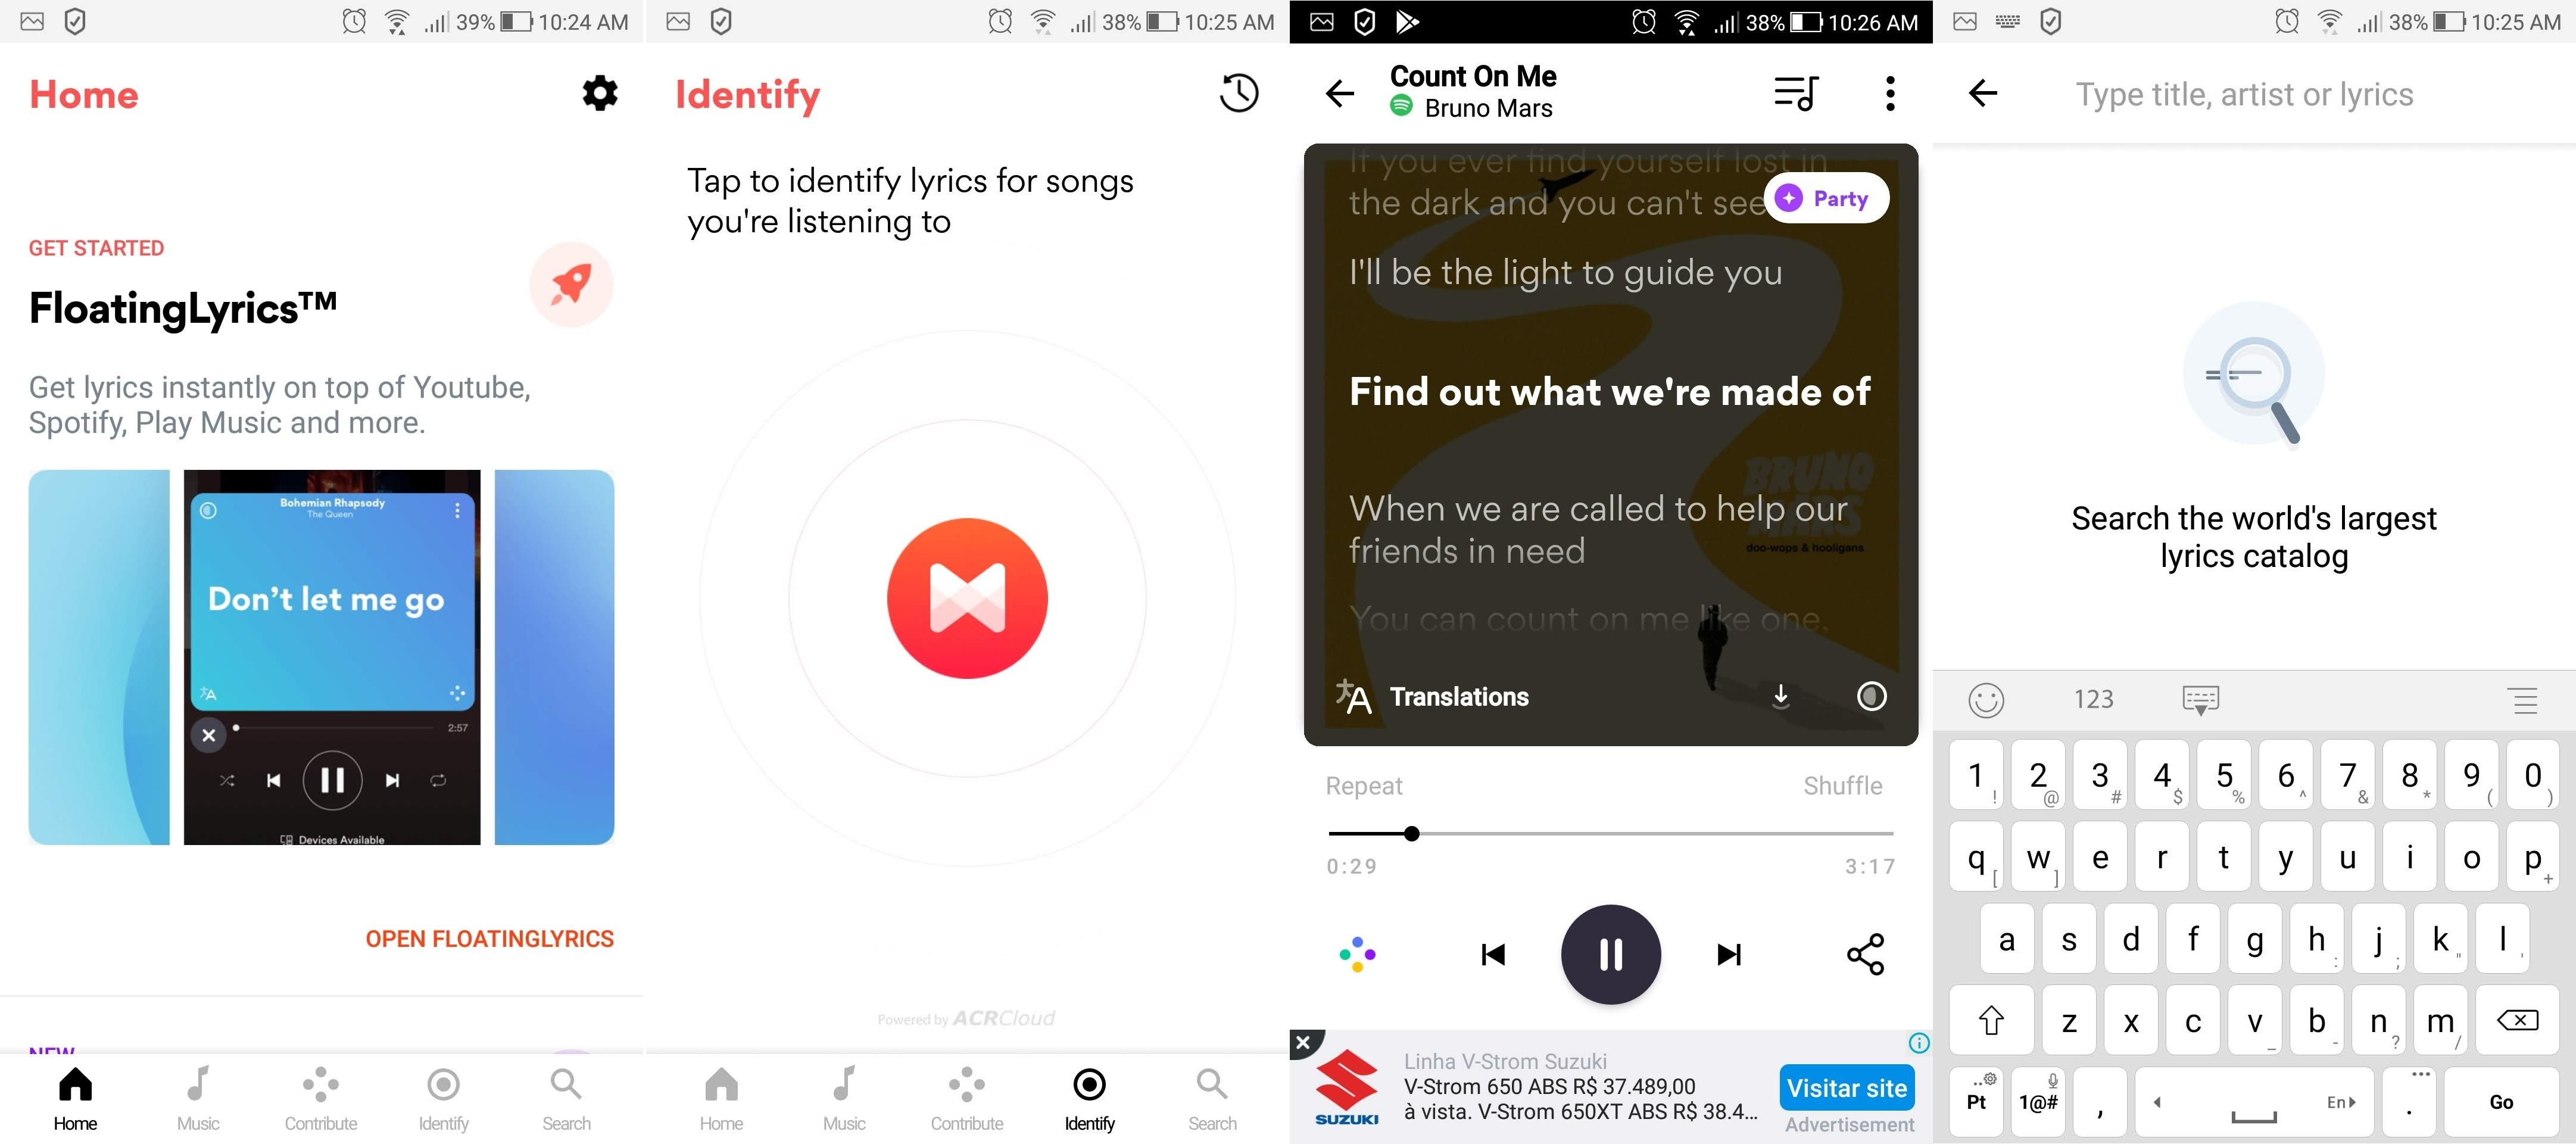
\includegraphics[scale=0.12]{figuras/musixmatch.jpg}
   \\Fonte: Elaborado pela autora
\end{figure}

%ACRCLOUD%
\subsection{ACRCloud} \label{subsec:acrcloud} %https://www.acrcloud.com/pt/music-recognition
A \textit{ACRCloud} foi criada em 2015, sendo a solução vitoriosa no campeonato de \textit{Audio Fingerprinting} do MIREX2015, organizado pelo Laboratório Internacional de Avaliação de Sistemas de Recuperação de Informação Musical (IMIRSEL, sigla em inglês).

ACR (\textit{Automatic Content Recognition}) é uma tecnologia de identificação para reconhecimento de conteúdo reproduzido em um dispositivo de mídia. Ele permite que usuários obtenham rapidamente informações detalhadas sobre o conteúdo que acabaram de experimentar sem qualquer entrada de texto ou esforço de pesquisa.

Segundo o site da companhia\footnote{https://www.acrcloud.com/docs/acrcloud/}, tradução nossa:

\begin{citacao}
O ACRCloud fornece serviços ACR em nuvem para ajudar empresas e desenvolvedores excelentes a criar aplicativos baseados em impressões digitais de áudio, como reconhecimento de áudio (suporte a música, vídeo, anúncios on-line e off-line), monitoramento de transmissão, interatividade de segunda tela, detecção de direitos autorais etc \cite{acrcloud2015}.
\end{citacao}

ACRCloud (ver Figura \ref{fig:acrcloud}) é uma plataforma de microserviços na nuvem que possui reconhecimento de música através de \textit{fingerprints}, onde identifica músicas ouvindo você cantar ou de músicas que são tocadas ao seu redor, além do monitoramento de transmissão com identificação e apresentação de conteúdo, entre outros. Ele possui integração com serviços de música como o Spotify, Deezer, entre outros, que permite desenvolvedores acessarem diretamente esses serviços e oferecer links diretos para seus usuários.

\begin{figure}[!htb]
   \centering
   \caption{ACRCloud}\label{fig:acrcloud} 
   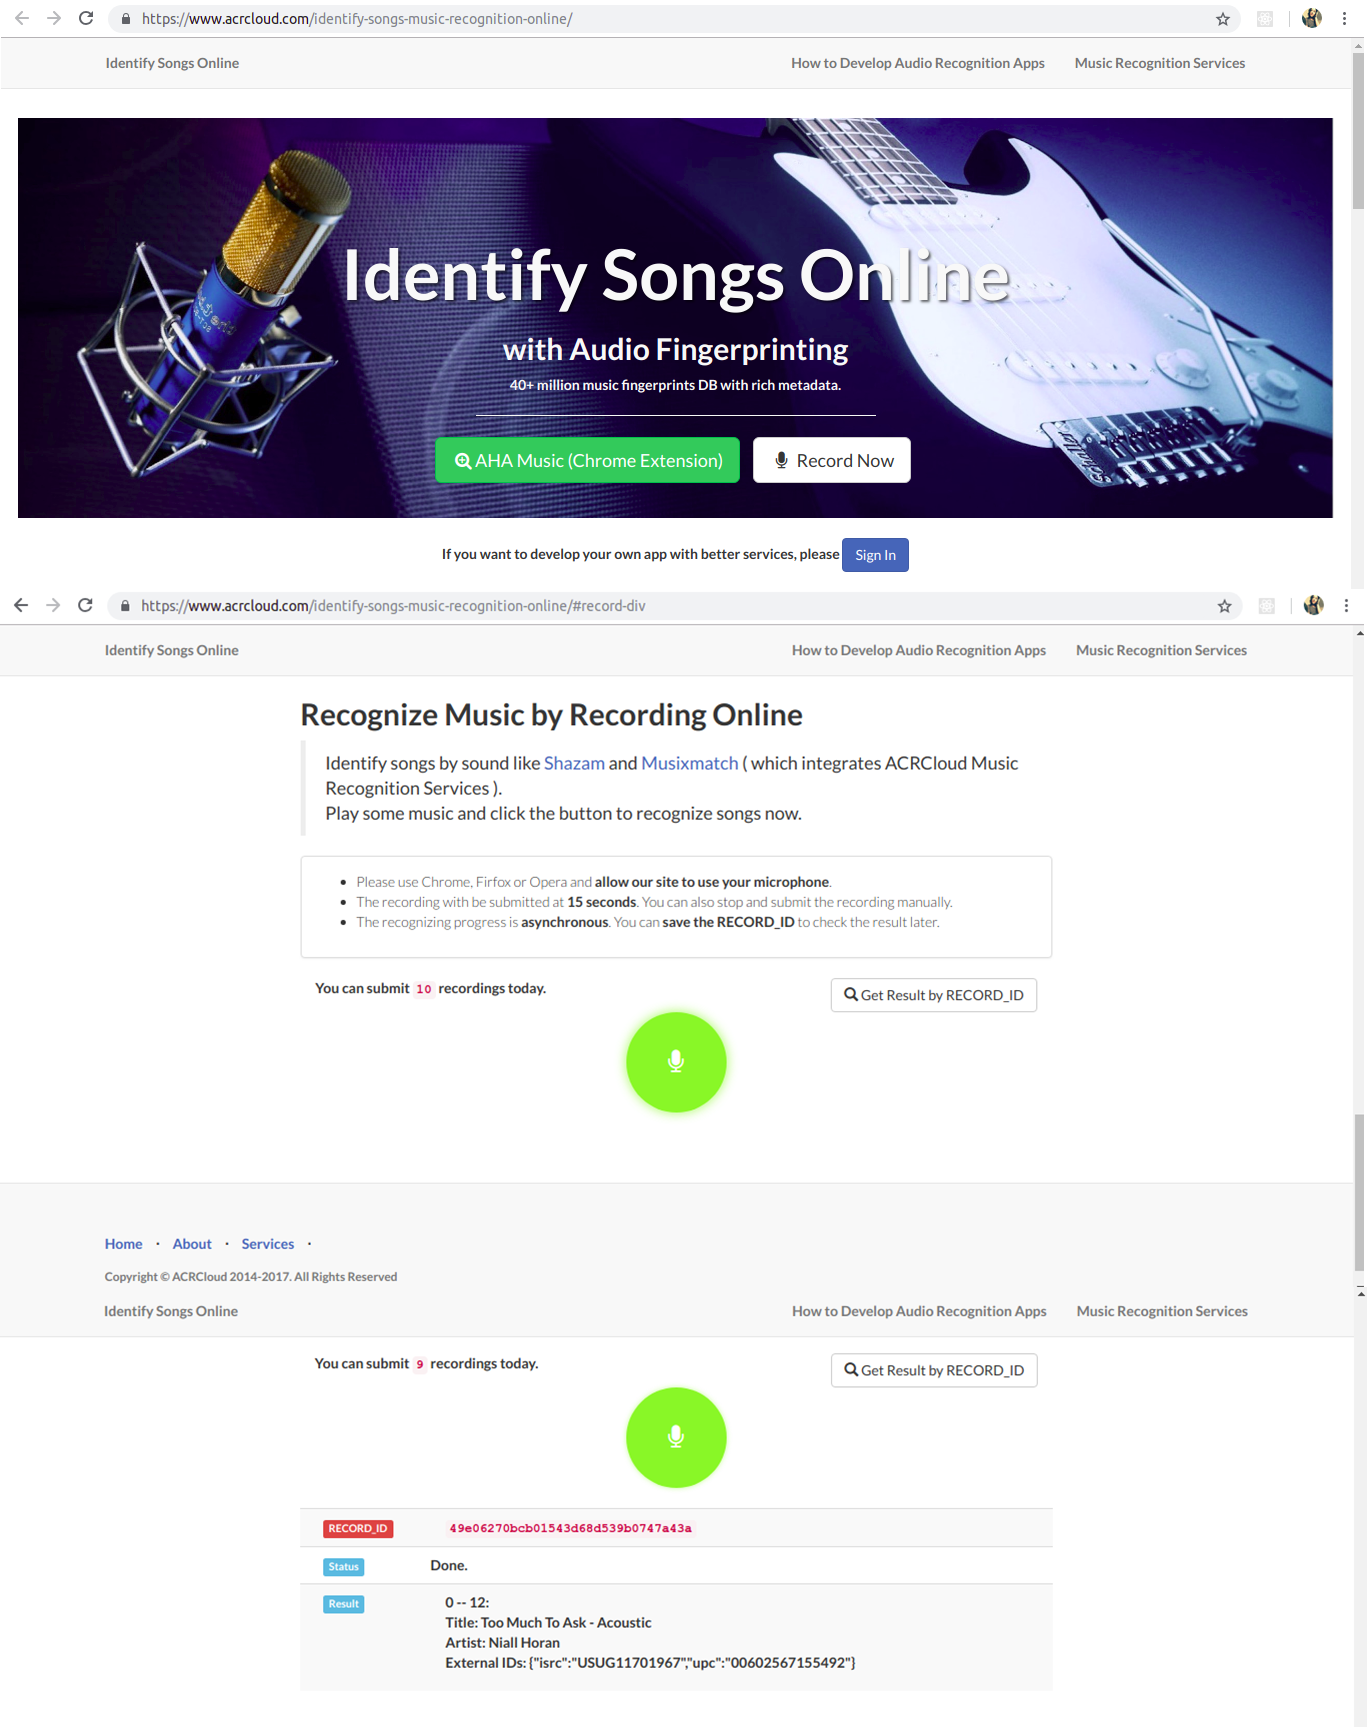
\includegraphics[scale=0.30]{figuras/acrcloud.png}
   \\Fonte: \cite{acrcloudSite}, elaborado pela autora
\end{figure}


%MUSIPEDIA%
\subsection{Musipedia} \label{subsec:musipedia}
Musipedia é uma enciclopédia aberta de música, criação inspirada no Wikipedia\footnote{https://www.wikipedia.org/}, para localização, edição e expansão de coleções de tons, melodias e temas musicais (ver Figura \ref{fig:musipedia}). A enciclopédia utiliza o mecanismo de pesquisa de melodias, do qual chamam de \textit{melodyhound}, onde é possível encontrar e identificar uma música, mesmo que a melodia seja tudo o que você saiba no momento. A busca também pode ser feita atavés da pesquisa de contorno melódico (Código de Pearson) ou com base no ritmo. Ainda, os conteúdos podem ser alterados por qualquer usuário, podendo conter um pedaço de música, um arquivo MIDI, informações textuais sobre o trabalho e o compositor.

A recuperação da informação, segundo o site da enciclopédia\footnote{https://www.musipedia.org/about.html}, pode ser feita da seguinte forma, tradução nossa:

\begin{citacao}
[...]Você pode tocá-lo em um teclado de piano, assobiar para o computador, simplesmente tocar o ritmo no teclado do computador ou usar o código Pearsons \cite{musipedia}.
\end{citacao}

É possível também integrar a pesquisa do Musipedia ao seu próprio serviço web, utilizando as interfaces SOAP, que possibilitam pesquisar com base na melodia, no contorno melódico ou no ritmo.

\begin{figure}[!htb]
   \centering
   \caption{Musipedia}\label{fig:musipedia} 
   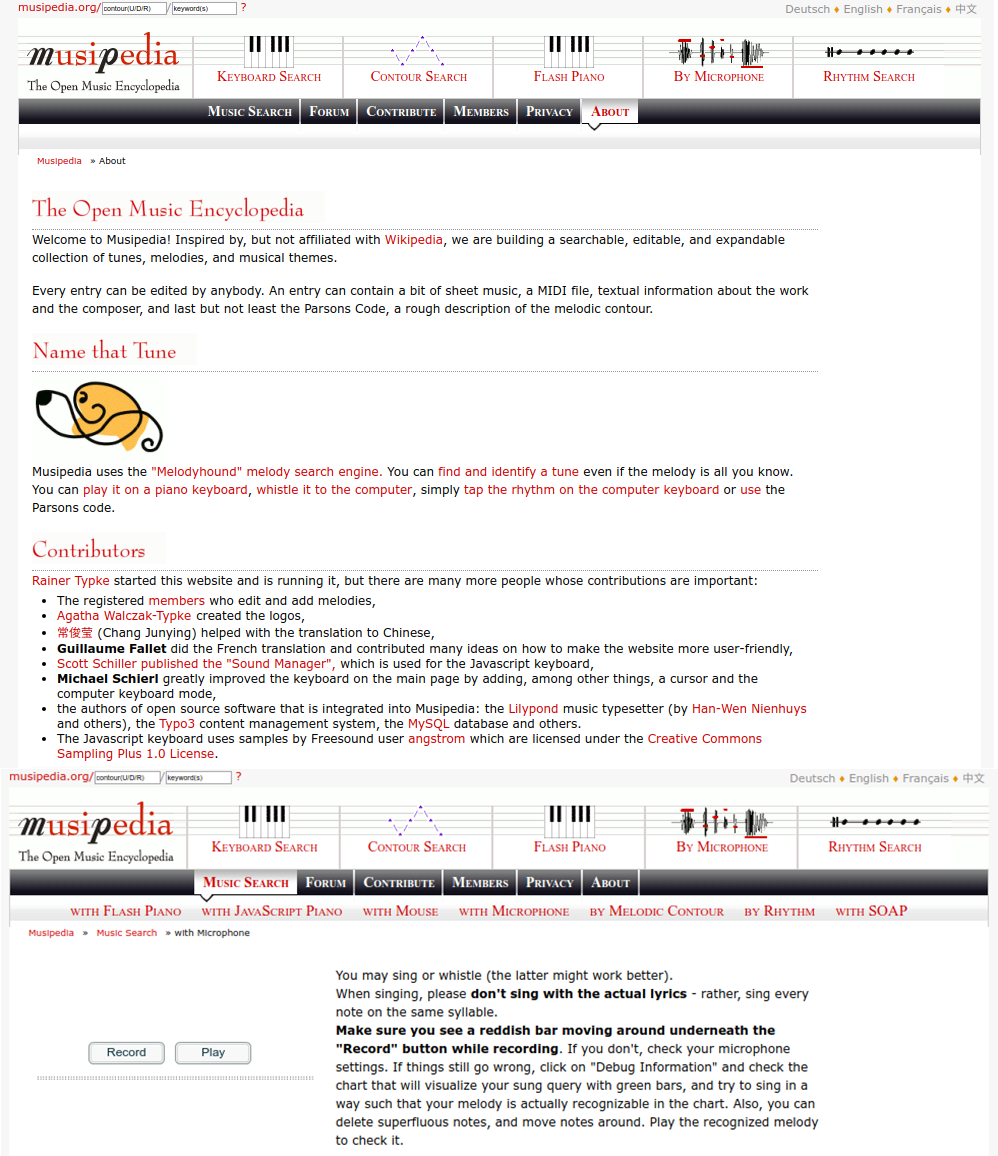
\includegraphics[scale=0.40]{figuras/musipedia.png}
   \\Fonte: \cite{musipedia}, elaborado pela autora
\end{figure}



%%ACADEMICO%%
\section{Acadêmico} \label{sec:academico}

%AMUSE%
\subsection{AMUSE} \label{subsec:amuse}
AMUSE (\textit{Advanced Music Explorer})\footnote{https://sourceforge.net/projects/amuse-framework/} é um \textit{framework} desenvolvido pela TU Dortmund, na Alemanha, licenciado sob a GPL e implementado em JAVA. Portanto, ele pode ser executado em qualquer sistema operacional que suporte o Java Runtime Environment (ver Figura \ref{fig:amuse}).

\begin{figure}[!htb]
   \centering
   \caption{AMUSE}\label{fig:amuse} 
   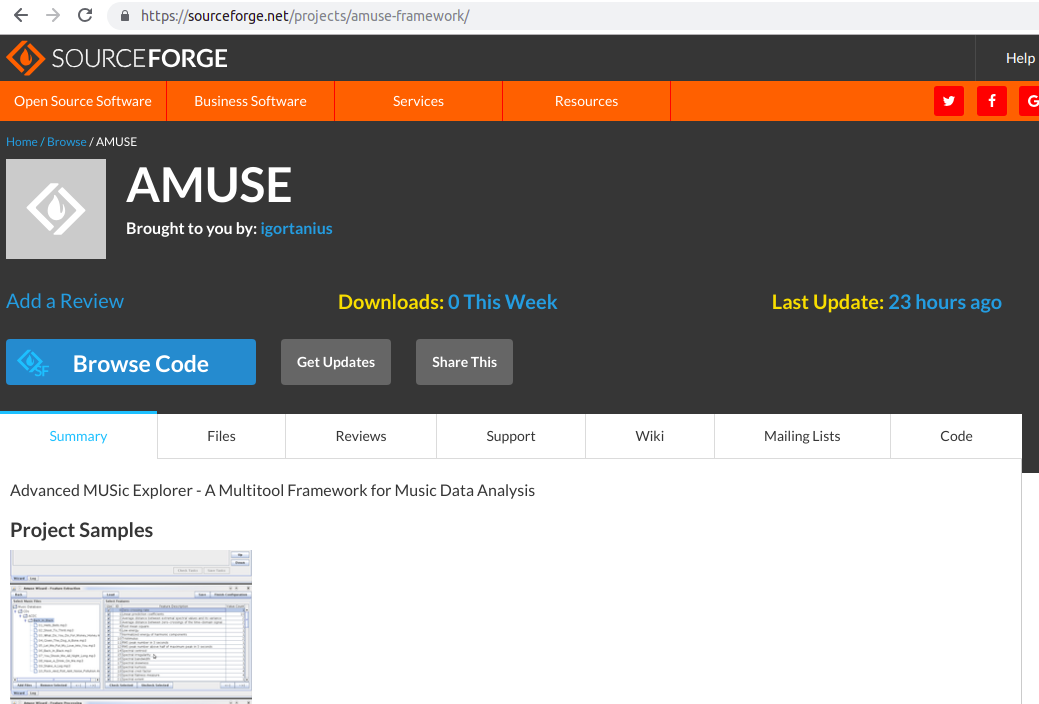
\includegraphics[scale=0.35]{figuras/amuse.png}
   \\Fonte: \cite{amuse}, elaborado pela autora
\end{figure}

Segundo \citeonline{vatolkin2010}, o \textit{framework} fornece diferentes funcionalidades, como:

\begin{itemize}
    \item Processamento de som, convertendo arquivos de áudio MP3 em ondas sonoras;
    \item \textit{Downsampling} e estéreo para a conversão de arquivos de áudio mono;
    \item Divisão automática de arquivos wave;
    \item Escalabilidade usando multi-threading em uma máquina ou fornecendo as tarefas para sistemas de grade como Sun Grid Engine ou LSF Batch;
    \item Gerenciamento eficiente do conjunto de dados que suporta diretamente o formato WEKA ARFF;
    \item Componente logger integrado.
\end{itemize}

O AMUSE possui subtarefas em cadeia para recuperação da informação musical. Cada tarefa pode ser calculada em várias unidades de processamento. Inicia-se pela tarefa de extração de recursos, que fornece descritores numéricos de baixo nível ou alto nível do sinal de áudio (por exemplo, extração de melodia da música). Depois que a tarefa de extração é carregada na memória, é realizado o processamento dos recursos, em uma etapa intermediária, que servirá de entrada para a técnica de classificação (ver subseção \ref{subsubsec:classificacao}). E por fim, a validação dos resultados da classificação. 

As ferramentas integradas não têm restrições de uso em relação aos seus códigos-fonte. Se eles não estiverem disponíveis como bibliotecas Java, as versões executáveis deverão ser fornecidas. Nesse caso, pode certamente levar à dependência do sistema operacional em execução.

O projeto é oferecido gratuitamente à comunidade de pesquisa. Informações mais detalhadas sobre o projeto podem ser consultadas em \cite{vatolkin2010} e \cite{amuse}.

%===>>> RONALDO - 29/10/2018: AQUI NO AMUSE TAMBEM SENTI FALTA DA EXPLICACAO DA TECNICA USADA PARA BUSCA POR SIMILARIDADE
%===>>> GISELE - 29/10/2018: ADICIONADO UM PARÁGRAFO SOBRE. VER SE FICOU BOA A EXPLICAÇÃO.

%CLAM%
\subsection{CLAM} \label{subsec:clam}
CLAM (\textit{C++ Library for Audio and Music})\footnote{http://clam-project.org/} é um \textit{framework} desenvolvido em C++ no \textit{Music Technology Group} (MTG) da Universidade Pompeu Fabra em Barcelona, Espanha. Ele oferece uma plataforma completa de desenvolvimento e pesquisa para o domínio de áudio e música, baseado na técnica SMS (ver subseção \ref{subsubsec:sms}). Além de oferecer um modelo abstrato para sistemas de áudio, ele também inclui um repositório de algoritmos de processamento e tipos de dados, bem como diversas ferramentas, como entrada/saída de áudio ou MIDI (ver Figura \ref{fig:clam}).

\begin{figure}[!htb]
   \centering
   \caption{CLAM}\label{fig:clam} 
   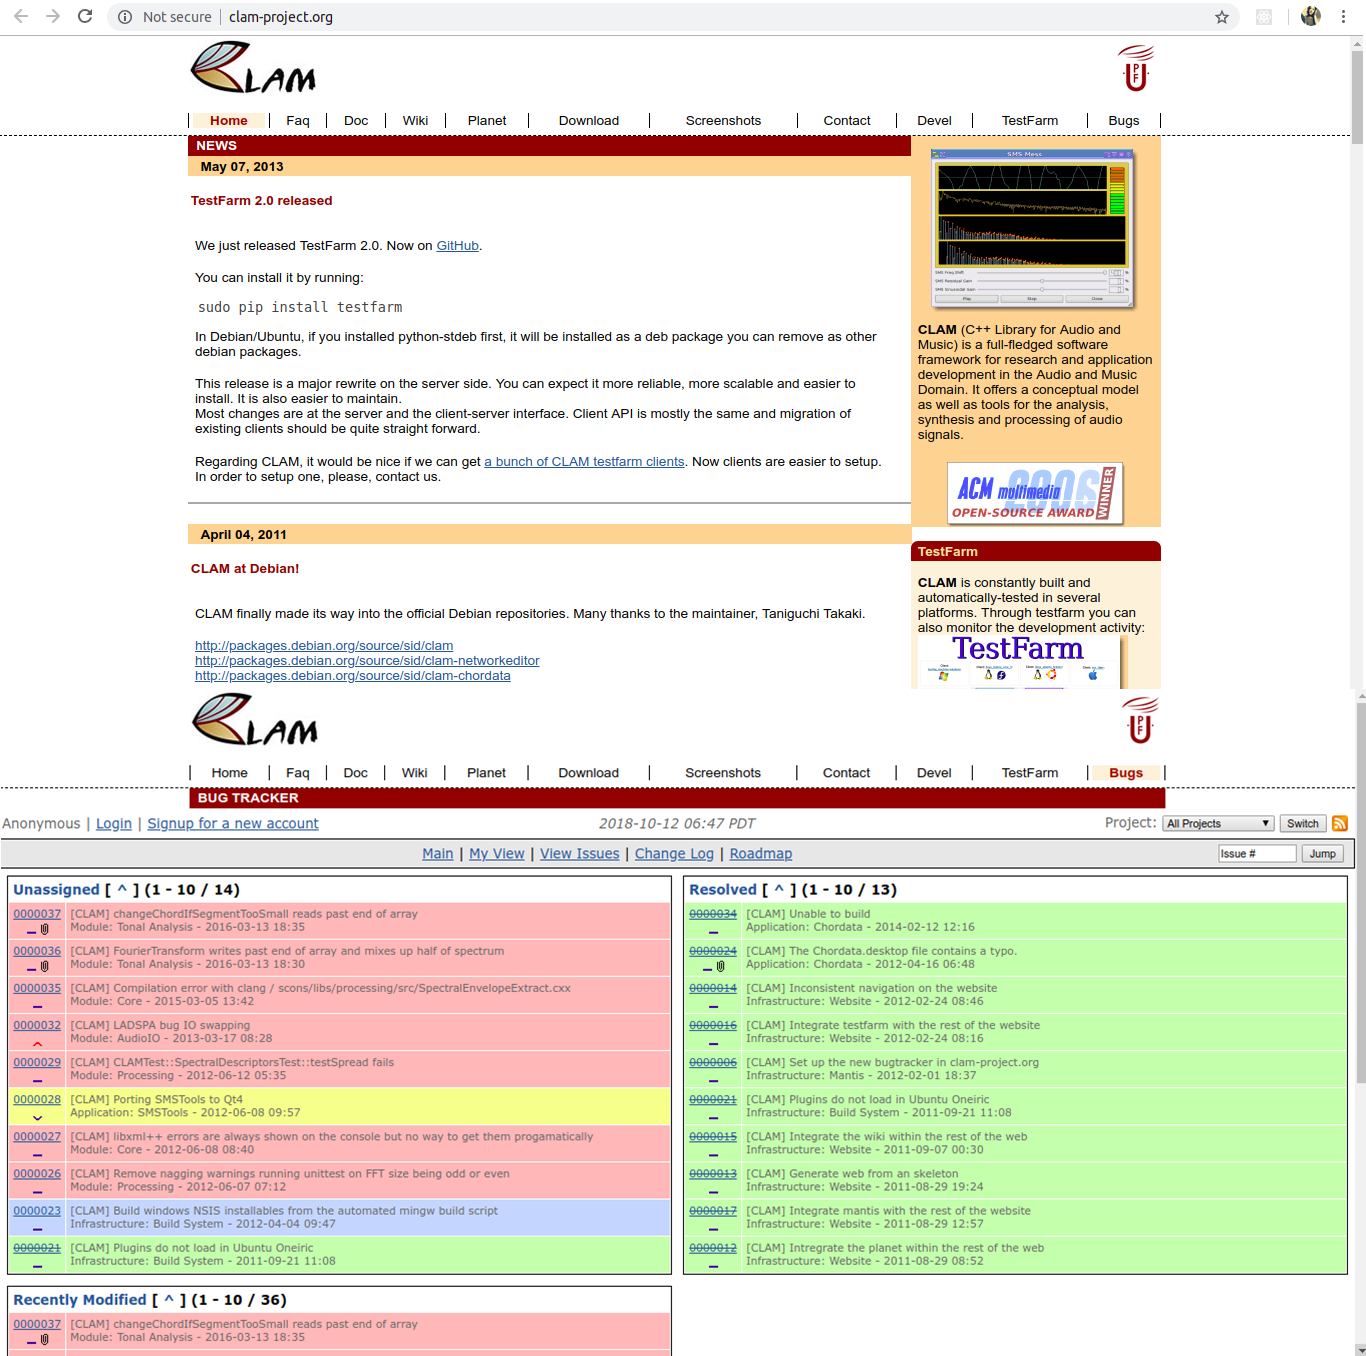
\includegraphics[scale=0.25]{figuras/clam.png}
   \\Fonte: \cite{clam}, elaborado pela autora
\end{figure}

Segundo \citeonline{amatriain2004}, as características mais importantes do framework são:

\begin{itemize}
    \item Verdadeiramente orientado a objetos. Extensas técnicas de engenharia de software foram aplicadas para projetar uma estrutura que seja altamente (re)utilizável e compreensível;
    \item É abrangente, uma vez que não só inclui classes para processamento, mas também para entrada e saída de áudio e MIDI, serviços de serialização XML, algoritmos e visualização e interação de dados, e manipulação multi-threading;
    \item Lida com uma ampla variedade de tipos de dados extensíveis que vão desde sinais de baixo nível (como áudio ou espectro) até estruturas semânticas de nível superior (como frase musical ou segmento);
    \item É multiplataforma. Todo o código é ANSI C ++ e é regularmente compilado no Linux, Windows e Mac OSX usando os compiladores mais usados. Até mesmo o código para entrada/saída, visualização e multithreading é de plataforma cruzada até a camada mais baixa possível;
    \item O projeto está licenciado sob os termos e condições GPL (Licença Pública GNU). Apesar de possuir a opção de licenciamento duplo da estrutura (ou seja, oferecer uma licença comercial alternativa), tudo o que é oferecido na versão pública é GPL e o projeto é, portanto, Software Livre, código aberto e colaborativo;
    \item Base para todos os desenvolvimentos futuros no MTG e, portanto, mantido e atualizado regularmente;
    \item O framework pode ser usado como uma biblioteca C ++ regular ou como uma ferramenta de prototipagem. No primeiro modo, o usuário pode estender, adaptar ou otimizar a funcionalidade da estrutura para implementar um aplicativo específico. No segundo modo, o usuário pode facilmente construir um protótipo para testar um novo algoritmo ou aplicativo de processamento de sinais.
\end{itemize}

Informações mais detalhadas sobre este \textit{framework} podem ser consultadas em \cite{amatriain2007, amatriain2004}.

%===>>> RONALDO - 29/10/2018: AQUI NO CLAM TAMBEM SENTI FALTA DA EXPLICACAO DA TECNICA USADA PARA BUSCA POR SIMILARIDADE
%===>>> GISELE - 29/10/2018: ADICIONADO NO PRIMEIRO PARAGRAFO. VER SE FICOU BOA A EXPLICAÇÃO.

%JAVA MIR%
\subsection{Java MIR} \label{subsec:jmir}
jMIR (Java MIR)\footnote{http://jmir.sourceforge.net/} é um \textit{software} que possui um conjunto de componentes desenvolvido na CIRMMT e Marianopolis College, ambos localizados no Canadá. Cada um dos componentes pode ser utilizado separadamente ou como um todo (ver Figura \ref{fig:jmir}).

%===>>> RONALDO - 29/10/2018: NO PARAGRAFO ACIMA INFORMAR QUAL EH O PAIS ONDE FICAM AS INSTITUICOES QUE DESENVOLVERAM O JMIR
%===>>> GISELE - 29/10/2018: FEITO

\begin{figure}[!htb]
   \centering
   \caption{Java MIR}\label{fig:jmir} 
   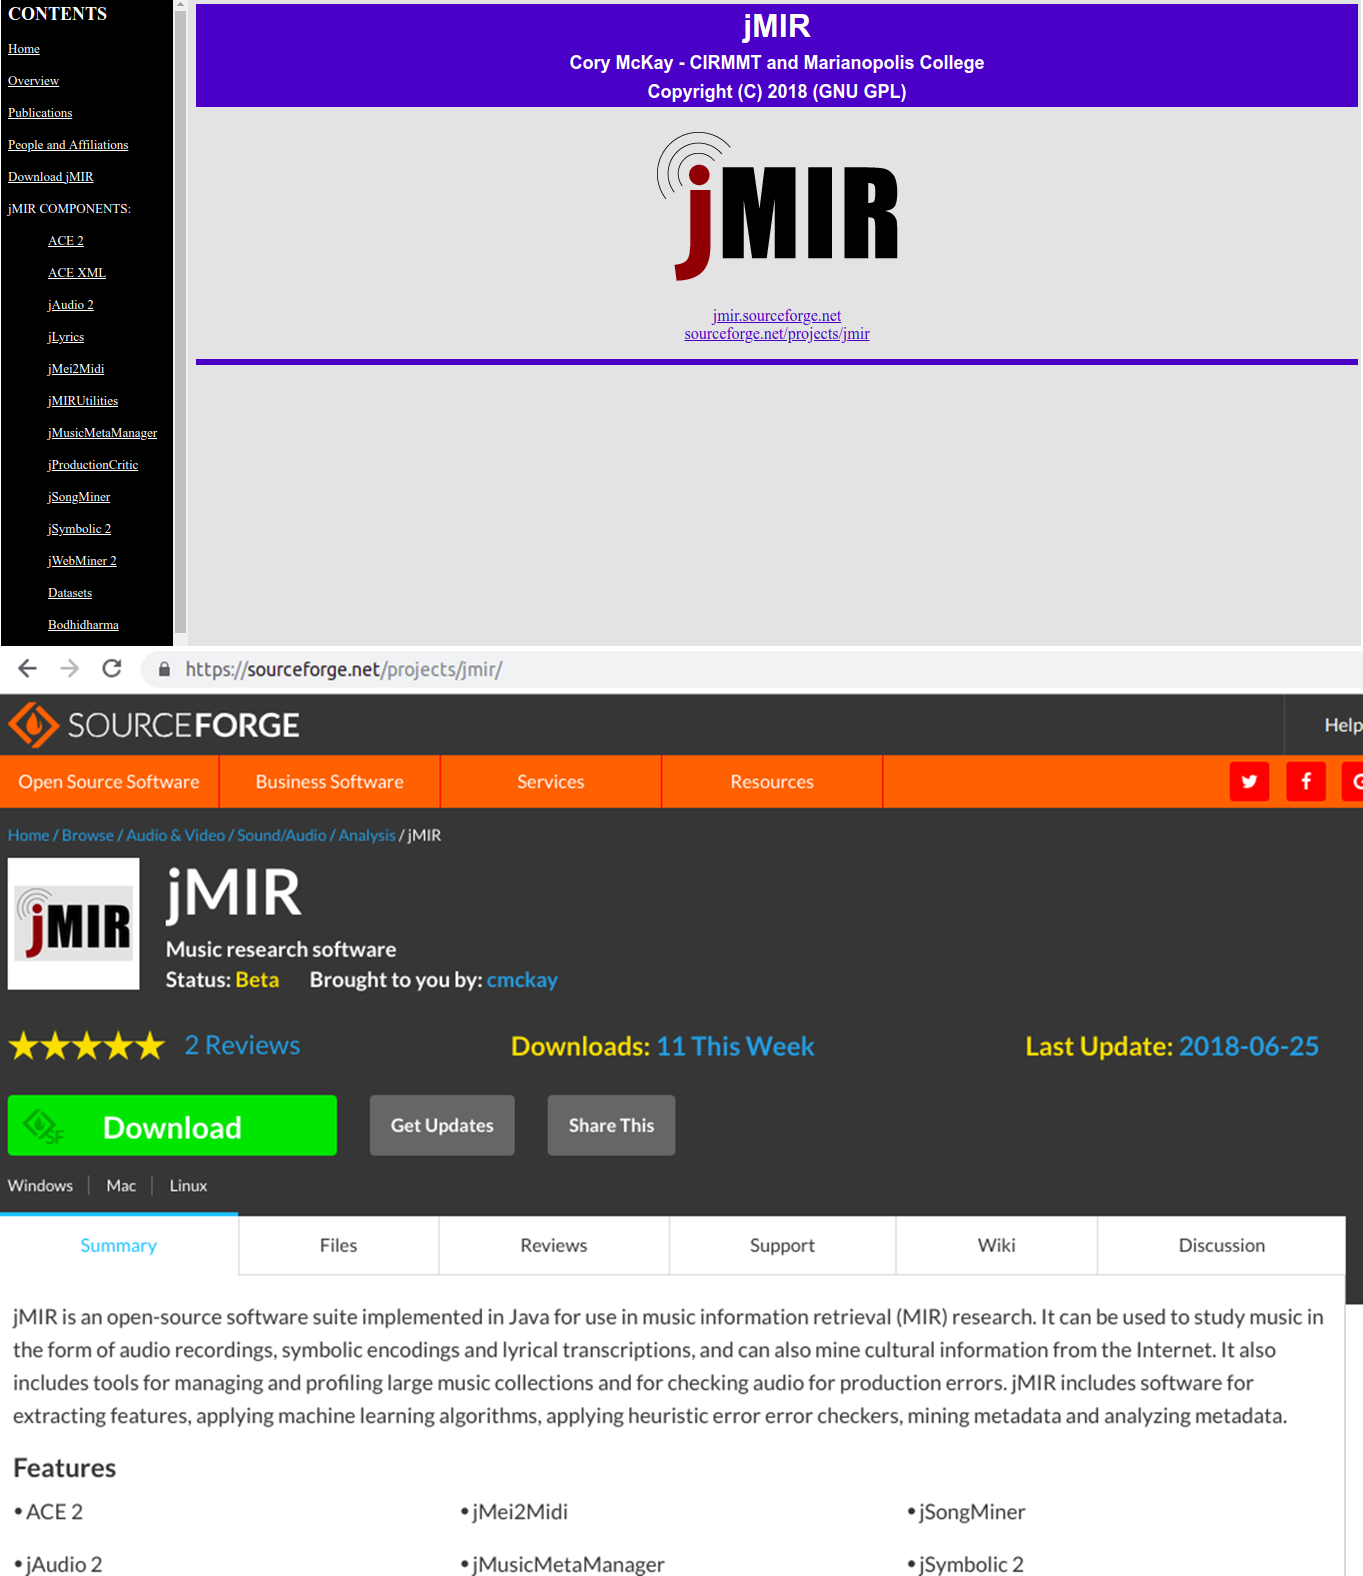
\includegraphics[scale=0.25]{figuras/jmir.png}
   \\Fonte: \cite{jmir}, elaborado pela autora
\end{figure}

O software é de código livre implementado em Java para uso nas pesquisas de Recuperação de Informação Musical (MIR), baseado em técnicas de mineração de dados, como a classificação (ver subseção \ref{subsubsec:classificacao}). Ele pode ser usado para estudar música na forma de gravações de áudio, codificações simbólicas e transcrições líricas, e também pode extrair informações culturais da Internet. Ainda, ele inclui ferramentas para gerenciar e criar perfis de grandes coleções de músicas e para verificar o áudio quanto a erros de produção. É bem documentado e inclui GUIs para aumentar a usabilidade geral.

O objetivo principal do \textit{software} é auxiliar nas pesquisas em classificação automática de música e a análise de similaridade, proporcionando as seguintes características:

\begin{itemize}
    \item Tornar tecnologias sofisticadas de reconhecimento de padrões acessíveis a pesquisadores de música com históricos técnicos e não técnicos;
    \item Eliminar duplicação redundante de esforço;
    \item Aumentar a cooperação e a comunicação entre os grupos de pesquisa;
    \begin{itemize}
        \item Facilitar o desenvolvimento iterativo e o compartilhamento de novas tecnologias MIR;
        \item Facilitar comparações objetivas de algoritmos.
    \end{itemize}
    \item Facilitar a pesquisa combinando características musicais de alto nível, baixo nível e culturais (ou seja, características simbólicas, áudio e web-minadas).
\end{itemize}

Informações mais detalhadas sobre o projeto estão disponíveis nas publicações acadêmicas\footnote{http://jmir.sourceforge.net/publications.html}. Manuais e documentação para cada componente também podem ser consultados em \cite{jmir} e \cite{mckay2010}.

%===>>> RONALDO - 29/10/2018: AQUI NO jMIR TAMBEM SENTI FALTA DA EXPLICACAO DA TECNICA USADA PARA BUSCA POR SIMILARIDADE
%===>>> GISELE - 29/10/2018: ADICIONADO NO SEGUNDO PARAGRAFO. VER SE FICOU BOA A EXPLICAÇÃO.

%MIR TOOLBOX%
\subsection{MIRtoolbox} \label{subsec:mirtoolbox}
\textit{MIRtoolbox}\footnote{https://www.jyu.fi/hytk/fi/laitokset/mutku/en/research/materials/mirtoolbox} é um pacote de ferramentas escritas em Matlab para a extração de recursos musicais, como tonalidade e ritmo, tanto para especialistas quanto para não especialistas do Matlab (ver Figura \ref{fig:mirtoolbox}). Ele foi desenvolvido dentro do contexto de um Projeto Europeu chamado “Tuning the Brain for Music”, dedicado ao estudo da música e da emoção, com colaboração entre neurociências, psicologia cognitiva e ciência da computação. Os grupos e instituições envolvidos são a Music Cognition Team da University of Jyväskylä na Finlândia e o Music Acoustics Group do KTH em Estocolmo.

\begin{figure}[!htb]
   \centering
   \caption{MIRtoolbox}\label{fig:mirtoolbox} 
   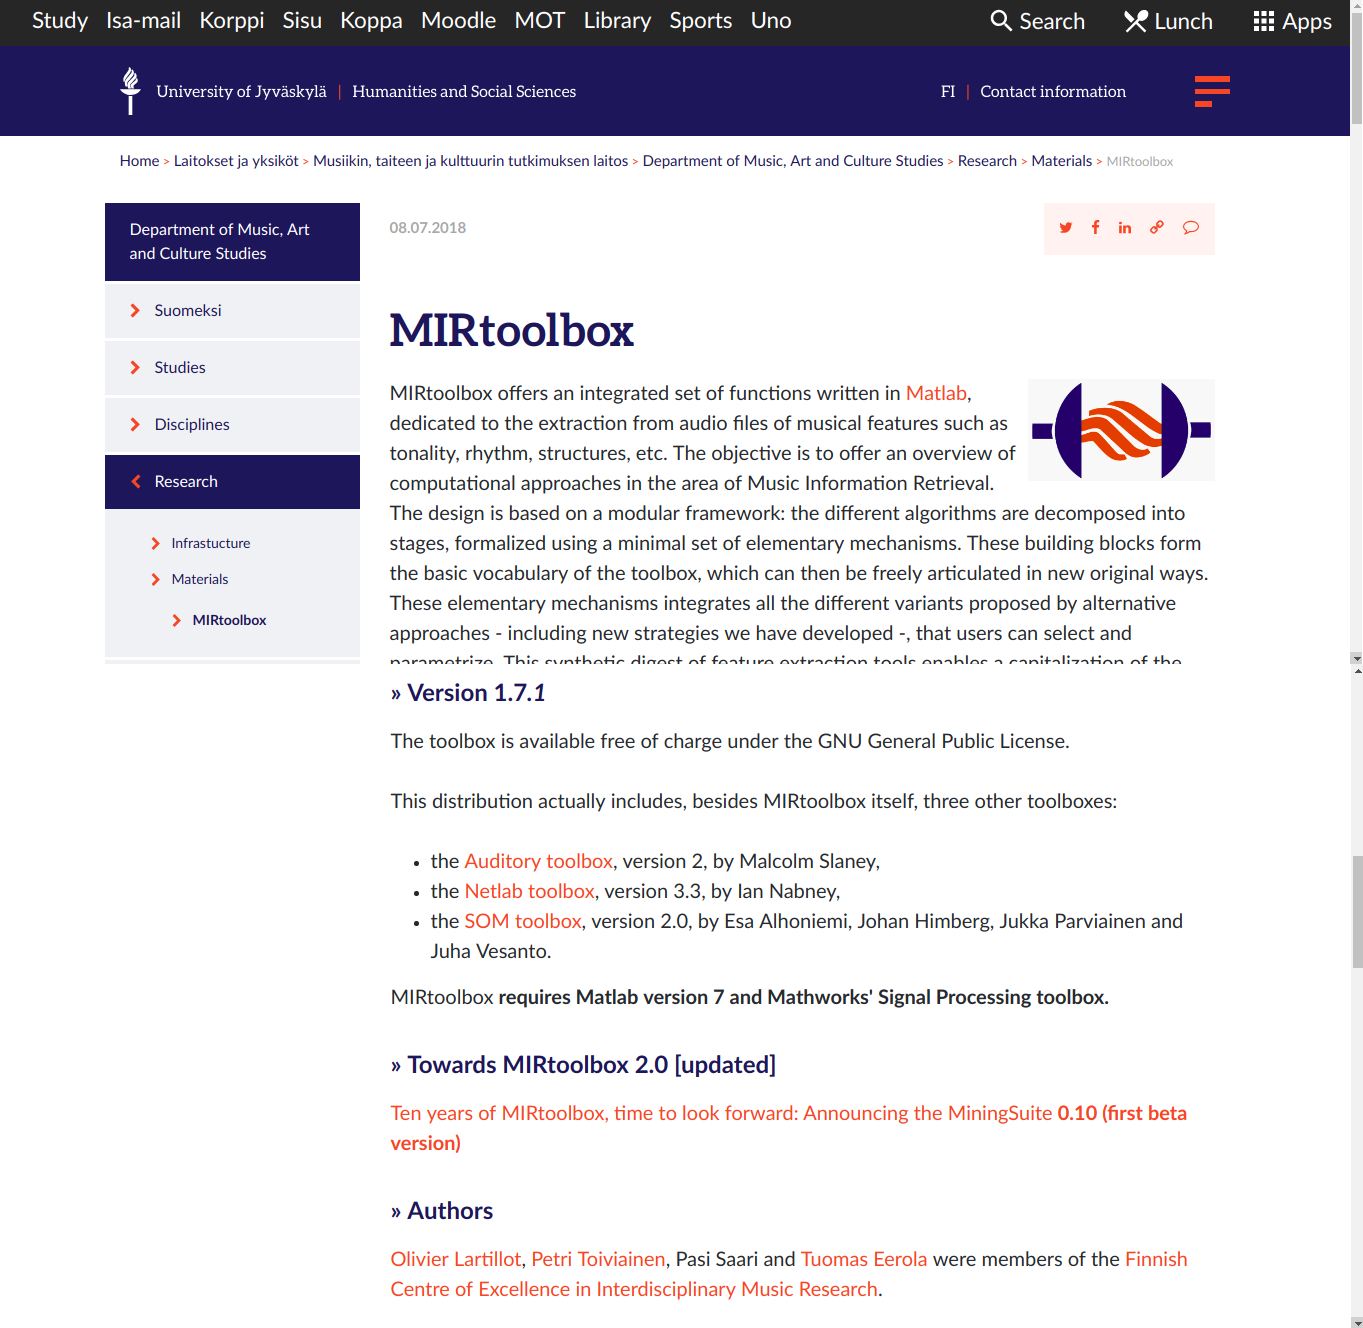
\includegraphics[scale=0.25]{figuras/mirtoolbox.png}
   \\Fonte: \cite{mirtoolbox}, elaborado pela autora
\end{figure}

Segundo \citeonline{lartillot2013}, foi elaborado um manual onde são descritas as seguintes especificações da solução:

\begin{itemize}
    \item Quadro modular: É baseado em um conjunto de blocos de construção que podem ser parametrizados, reutilizados, reordenados, etc.;
    \item Sintaxe simples e adaptativa: Os usuários podem se concentrar no design geral e o MIRtoolbox que cuida das tarefas laboriosas subjacentes;
    \item Software livre e código-fonte aberto: A ideia é propor a capitalização da expertise da comunidade de pesquisa e oferecê-la de volta à comunidade;
    \item Recursos: O MIRtoolbox inclui cerca de 50 extratores de recursos de áudio e música e descritores estatísticos.
\end{itemize}

O MIRtoolbox é baseado em técnicas de mineração de dados, e por ser um pacote de ferramentas, são variadas técnicas para recuperação da informação musical, entre elas podemos citar: clusterização (ver subseção \ref{subsubsec:clustering}) e classificação (ver subseção \ref{subsubsec:classificacao}).

Desta forma, ele pode ser útil para a comunidade de pesquisa em Recuperação da Informação Musical (MIR), mas também para fins educacionais. Mais informações sobre o projeto podem ser consultadas em \cite{lartillot2007, lartillot2013} e \cite{mirtoolbox}

%===>>> RONALDO - 29/10/2018: AQUI NO MIRTOOLBOX TAMBEM SENTI FALTA DA EXPLICACAO DA TECNICA USADA PARA BUSCA POR SIMILARIDADE
%===>>> GISELE - 29/10/2018: ADICIONADO UM PARÁGRAFO.

%MUSIC MINER%
\subsection{MusicMiner} \label{subsec:musicminer}
O \textit{Databionic MusicMiner}, desenvolvido como parte de um projeto de pesquisa do Grupo de Pesquisa em Databionics da Universidade de Marburg, na Alemanha, é um navegador para dados musicais baseado em técnicas de mineração de dados, como clusterização (ver subseção \ref{subsubsec:clustering}) e visualização (ver subseção \ref{subsubsec:visualizacao}) com base no paradigma dos mapas geográficos ESOM  (ver Figura \ref{fig:musicminer}).

\begin{figure}[!htb]
   \centering
   \caption{MusicMiner}\label{fig:musicminer} 
   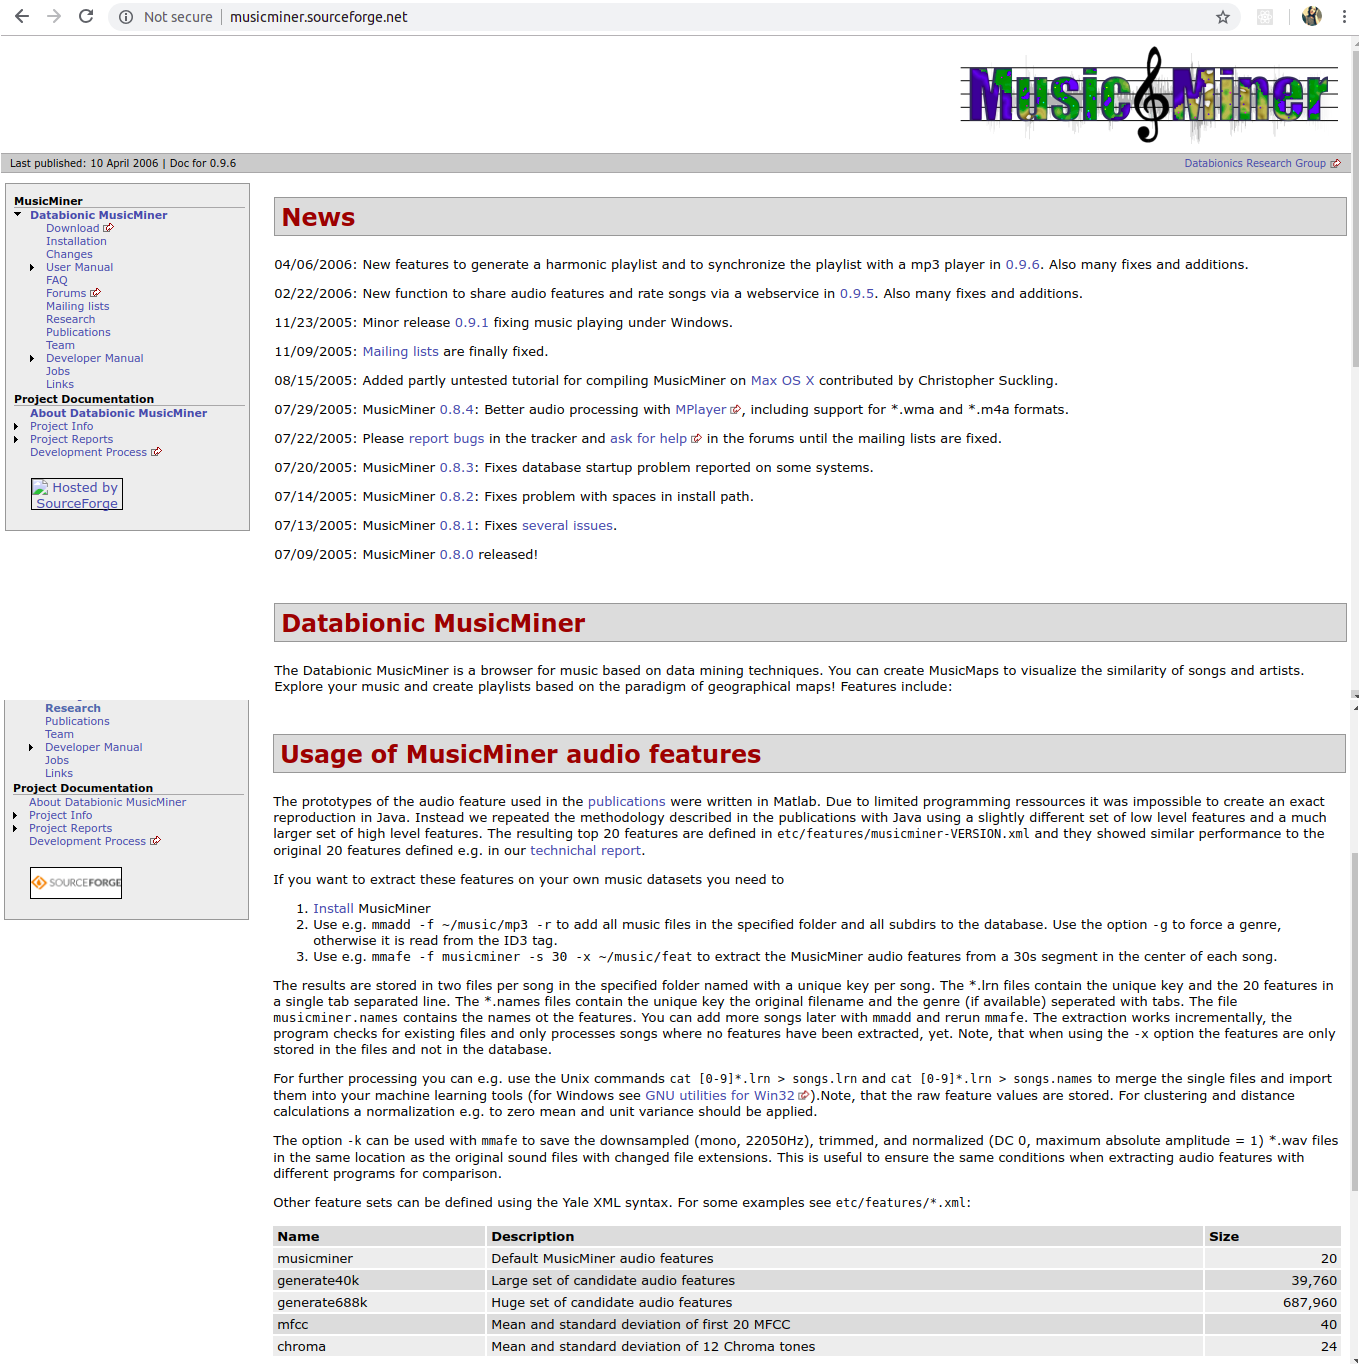
\includegraphics[scale=0.25]{figuras/musicminer.png}
   \\Fonte: \cite{musicminer}, elaborado pela autora
\end{figure}

A coleção de músicas é recuperada e apresentada em forma de mapa topográfico com pequenos pontos para as músicas. O usuário pode interagir com o mapa de diferentes formas para selecionar e ouvir músicas; explorar suas músicas; e criar playlists baseadas no paradigma de mapas geográficos.

O site do projeto\footnote{http://musicminer.sourceforge.net/}  apresenta as seguintes características da solução:

\begin{itemize}
    \item Análise automática de uma árvore de pastas com arquivos de música (MP3, OGG, WMA, M4A, MP2, WAV);
    \item Descrição automática de arquivos de áudio digital por som;
    \item Criação de \textit{MusicMaps} para navegar pelo espaço sonoro com base no paradigma dos mapas geográficos ESOM;
    \item Criação visual de \textit{playlists};
    \item Pesquisa por similaridade na coleção de músicas com base no som;
    \item Navegação hierárquica personalizável da base de dados, como por exemplo, por gênero/artista/álbum ou ano/artista;
    \item Base de dados flexível, incluindo o armazenamento separado de vários artistas por música, álbuns e listas de reprodução como parte de uma lista de reprodução;
    \item Importação e exportação de meta informações baseadas em XML.
\end{itemize}

O \textit{MusicMiner} é escrito em Java para máxima portabilidade e publicado sob os termos da GPL (General Public License). Seu foco principal é a pesquisa e o ensino. Informações mais detalhadas sobre o projeto podem ser encontradas em \cite{morchen2005} e \cite{musicminer}.

%TUNEBOT%
\subsection{Tunebot} \label{subsec:tunebot}
\textit{Tunebot}\footnote{http://music.cs.northwestern.edu/data/tunebot/} é um projeto criado em 2015, desenvolvido e mantido por \textit{Interactive Audio Lab}\footnote{http://music.eecs.northwestern.edu/} na Universidade de Northwestern, nos Estados Unidos. Segundo \citeonline{pardo2010}, o Tunebot está disponível como um serviço web (ver Figura \ref{fig:tunebotWeb}) e está atualmente em teste beta como um aplicativo do iPhone (ver Figura \ref{fig:tunebotIphone}). A interação do usuário nas versões da Web e do iPhone é idêntica:
(i) cante, e (ii) escolha. O usuário simplesmente canta uma parte da música desejada para o Tunebot e o sistema retorna uma lista ordenada de músicas. Cada música pode ser reproduzida por um simples clique. Enquanto a música está tocando, o sistema apresenta uma caixa de diálogo perguntando se esta é a música correta. Se o usuário clicar em "sim", a consulta será armazenada no banco de dados como um exemplo pesquisável para essa música. O usuário é conectado à Amazon.com ou ao iTunes, onde a música pode ser comprada.

\begin{figure}[!htb]
   \centering
   \caption{Aplicativo Tunebot}\label{fig:tunebotIphone} 
   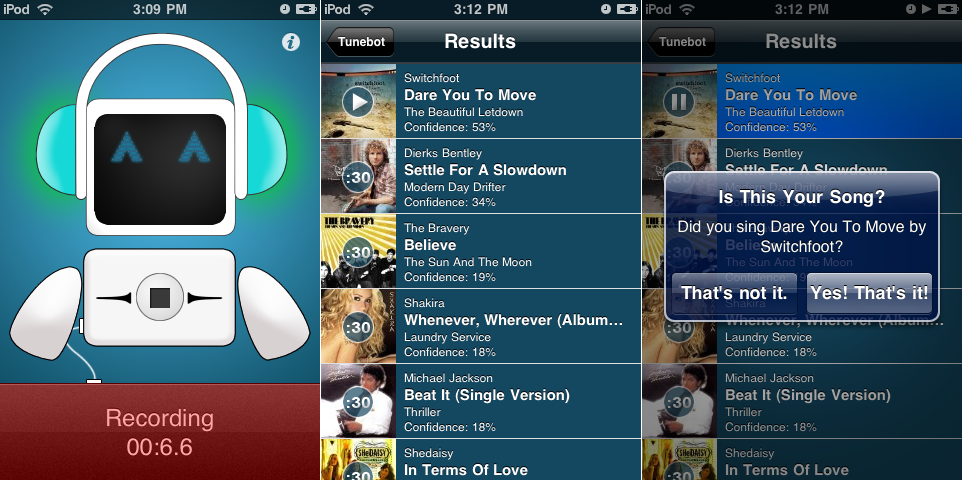
\includegraphics[scale=0.35]{figuras/tunebot-iphone.png}
   \\Fonte: \cite{tunebotiOS}, elaborado pela autora
\end{figure}

\begin{figure}[!htb]
   \centering
   \caption{Tunebot Web}\label{fig:tunebotWeb} 
   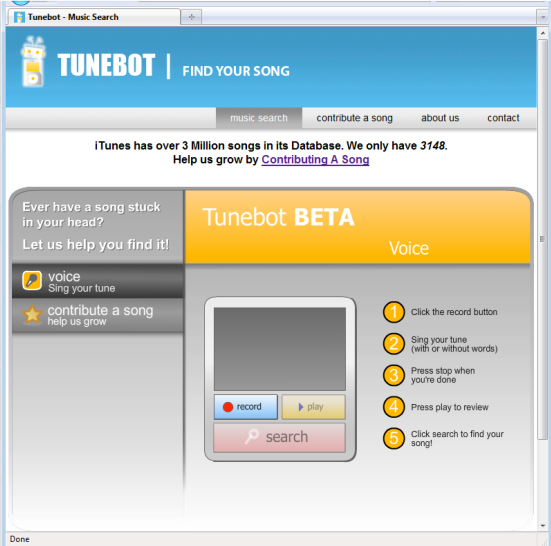
\includegraphics[scale=0.50]{figuras/tunebotWeb.png}
   \\Fonte: \cite{pardo2010}
\end{figure}

O sistema não exige chaves de pesquisa codificadas manualmente, pois atualiza automaticamente o banco de dados com novas chaves de pesquisa derivadas de consultas e contribuições do usuário \cite{pardo2010}. O banco de dados do \textit{Tunebot} compara as músicas com as músicas cantadas pelos usuários utilizando o algoritmo \textit{query by humming} (ver subseção \ref{subsubsec:qbh}).

Outro objetivo do projeto é ajudar pesquisadores na área de reconhecimento de músicas que utilizam o algoritmo \textit{query by humming}, facilitando uma pesquisa mais precisa do desempenho do mundo real do que seria possível com conjuntos de dados existentes.

Informações mais detalhadas sobre o projeto podem ser consultadas em \cite{pardo2010, pardo2012} e \cite{huq2010}.


